% Options for packages loaded elsewhere
\PassOptionsToPackage{unicode}{hyperref}
\PassOptionsToPackage{hyphens}{url}
%
\documentclass[
]{article}
\usepackage{lmodern}
\usepackage{amssymb,amsmath}
\usepackage{ifxetex,ifluatex}
\ifnum 0\ifxetex 1\fi\ifluatex 1\fi=0 % if pdftex
  \usepackage[T1]{fontenc}
  \usepackage[utf8]{inputenc}
  \usepackage{textcomp} % provide euro and other symbols
\else % if luatex or xetex
  \usepackage{unicode-math}
  \defaultfontfeatures{Scale=MatchLowercase}
  \defaultfontfeatures[\rmfamily]{Ligatures=TeX,Scale=1}
\fi
% Use upquote if available, for straight quotes in verbatim environments
\IfFileExists{upquote.sty}{\usepackage{upquote}}{}
\IfFileExists{microtype.sty}{% use microtype if available
  \usepackage[]{microtype}
  \UseMicrotypeSet[protrusion]{basicmath} % disable protrusion for tt fonts
}{}
\makeatletter
\@ifundefined{KOMAClassName}{% if non-KOMA class
  \IfFileExists{parskip.sty}{%
    \usepackage{parskip}
  }{% else
    \setlength{\parindent}{0pt}
    \setlength{\parskip}{6pt plus 2pt minus 1pt}}
}{% if KOMA class
  \KOMAoptions{parskip=half}}
\makeatother
\usepackage{xcolor}
\IfFileExists{xurl.sty}{\usepackage{xurl}}{} % add URL line breaks if available
\IfFileExists{bookmark.sty}{\usepackage{bookmark}}{\usepackage{hyperref}}
\hypersetup{
  pdftitle={Statistical Learning Project},
  pdfauthor={Andrea Ierardi},
  hidelinks,
  pdfcreator={LaTeX via pandoc}}
\urlstyle{same} % disable monospaced font for URLs
\usepackage[margin=1in]{geometry}
\usepackage{color}
\usepackage{fancyvrb}
\newcommand{\VerbBar}{|}
\newcommand{\VERB}{\Verb[commandchars=\\\{\}]}
\DefineVerbatimEnvironment{Highlighting}{Verbatim}{commandchars=\\\{\}}
% Add ',fontsize=\small' for more characters per line
\usepackage{framed}
\definecolor{shadecolor}{RGB}{248,248,248}
\newenvironment{Shaded}{\begin{snugshade}}{\end{snugshade}}
\newcommand{\AlertTok}[1]{\textcolor[rgb]{0.94,0.16,0.16}{#1}}
\newcommand{\AnnotationTok}[1]{\textcolor[rgb]{0.56,0.35,0.01}{\textbf{\textit{#1}}}}
\newcommand{\AttributeTok}[1]{\textcolor[rgb]{0.77,0.63,0.00}{#1}}
\newcommand{\BaseNTok}[1]{\textcolor[rgb]{0.00,0.00,0.81}{#1}}
\newcommand{\BuiltInTok}[1]{#1}
\newcommand{\CharTok}[1]{\textcolor[rgb]{0.31,0.60,0.02}{#1}}
\newcommand{\CommentTok}[1]{\textcolor[rgb]{0.56,0.35,0.01}{\textit{#1}}}
\newcommand{\CommentVarTok}[1]{\textcolor[rgb]{0.56,0.35,0.01}{\textbf{\textit{#1}}}}
\newcommand{\ConstantTok}[1]{\textcolor[rgb]{0.00,0.00,0.00}{#1}}
\newcommand{\ControlFlowTok}[1]{\textcolor[rgb]{0.13,0.29,0.53}{\textbf{#1}}}
\newcommand{\DataTypeTok}[1]{\textcolor[rgb]{0.13,0.29,0.53}{#1}}
\newcommand{\DecValTok}[1]{\textcolor[rgb]{0.00,0.00,0.81}{#1}}
\newcommand{\DocumentationTok}[1]{\textcolor[rgb]{0.56,0.35,0.01}{\textbf{\textit{#1}}}}
\newcommand{\ErrorTok}[1]{\textcolor[rgb]{0.64,0.00,0.00}{\textbf{#1}}}
\newcommand{\ExtensionTok}[1]{#1}
\newcommand{\FloatTok}[1]{\textcolor[rgb]{0.00,0.00,0.81}{#1}}
\newcommand{\FunctionTok}[1]{\textcolor[rgb]{0.00,0.00,0.00}{#1}}
\newcommand{\ImportTok}[1]{#1}
\newcommand{\InformationTok}[1]{\textcolor[rgb]{0.56,0.35,0.01}{\textbf{\textit{#1}}}}
\newcommand{\KeywordTok}[1]{\textcolor[rgb]{0.13,0.29,0.53}{\textbf{#1}}}
\newcommand{\NormalTok}[1]{#1}
\newcommand{\OperatorTok}[1]{\textcolor[rgb]{0.81,0.36,0.00}{\textbf{#1}}}
\newcommand{\OtherTok}[1]{\textcolor[rgb]{0.56,0.35,0.01}{#1}}
\newcommand{\PreprocessorTok}[1]{\textcolor[rgb]{0.56,0.35,0.01}{\textit{#1}}}
\newcommand{\RegionMarkerTok}[1]{#1}
\newcommand{\SpecialCharTok}[1]{\textcolor[rgb]{0.00,0.00,0.00}{#1}}
\newcommand{\SpecialStringTok}[1]{\textcolor[rgb]{0.31,0.60,0.02}{#1}}
\newcommand{\StringTok}[1]{\textcolor[rgb]{0.31,0.60,0.02}{#1}}
\newcommand{\VariableTok}[1]{\textcolor[rgb]{0.00,0.00,0.00}{#1}}
\newcommand{\VerbatimStringTok}[1]{\textcolor[rgb]{0.31,0.60,0.02}{#1}}
\newcommand{\WarningTok}[1]{\textcolor[rgb]{0.56,0.35,0.01}{\textbf{\textit{#1}}}}
\usepackage{graphicx,grffile}
\makeatletter
\def\maxwidth{\ifdim\Gin@nat@width>\linewidth\linewidth\else\Gin@nat@width\fi}
\def\maxheight{\ifdim\Gin@nat@height>\textheight\textheight\else\Gin@nat@height\fi}
\makeatother
% Scale images if necessary, so that they will not overflow the page
% margins by default, and it is still possible to overwrite the defaults
% using explicit options in \includegraphics[width, height, ...]{}
\setkeys{Gin}{width=\maxwidth,height=\maxheight,keepaspectratio}
% Set default figure placement to htbp
\makeatletter
\def\fps@figure{htbp}
\makeatother
\setlength{\emergencystretch}{3em} % prevent overfull lines
\providecommand{\tightlist}{%
  \setlength{\itemsep}{0pt}\setlength{\parskip}{0pt}}
\setcounter{secnumdepth}{-\maxdimen} % remove section numbering

\title{Statistical Learning Project}
\author{Andrea Ierardi}
\date{}

\begin{document}
\maketitle

pdf\_document: default html\_document: default

\hypertarget{libraries}{%
\section{Libraries}\label{libraries}}

\begin{Shaded}
\begin{Highlighting}[]
\KeywordTok{library}\NormalTok{(knitr)}
\KeywordTok{library}\NormalTok{(ggplot2)}
\end{Highlighting}
\end{Shaded}

\begin{verbatim}
## Warning: package 'ggplot2' was built under R version 3.6.3
\end{verbatim}

\begin{Shaded}
\begin{Highlighting}[]
\KeywordTok{library}\NormalTok{(plotly)}
\end{Highlighting}
\end{Shaded}

\begin{verbatim}
## Warning: package 'plotly' was built under R version 3.6.3
\end{verbatim}

\begin{verbatim}
## 
## Attaching package: 'plotly'
\end{verbatim}

\begin{verbatim}
## The following object is masked from 'package:ggplot2':
## 
##     last_plot
\end{verbatim}

\begin{verbatim}
## The following object is masked from 'package:stats':
## 
##     filter
\end{verbatim}

\begin{verbatim}
## The following object is masked from 'package:graphics':
## 
##     layout
\end{verbatim}

\begin{Shaded}
\begin{Highlighting}[]
\KeywordTok{library}\NormalTok{(tidyr)}
\KeywordTok{library}\NormalTok{(dplyr)}
\end{Highlighting}
\end{Shaded}

\begin{verbatim}
## Warning: package 'dplyr' was built under R version 3.6.3
\end{verbatim}

\begin{verbatim}
## 
## Attaching package: 'dplyr'
\end{verbatim}

\begin{verbatim}
## The following objects are masked from 'package:stats':
## 
##     filter, lag
\end{verbatim}

\begin{verbatim}
## The following objects are masked from 'package:base':
## 
##     intersect, setdiff, setequal, union
\end{verbatim}

\begin{Shaded}
\begin{Highlighting}[]
\KeywordTok{library}\NormalTok{(png)}
\KeywordTok{library}\NormalTok{(ggpubr)}
\end{Highlighting}
\end{Shaded}

\begin{verbatim}
## Warning: package 'ggpubr' was built under R version 3.6.3
\end{verbatim}

\begin{Shaded}
\begin{Highlighting}[]
\KeywordTok{library}\NormalTok{(tidyverse)}
\end{Highlighting}
\end{Shaded}

\begin{verbatim}
## -- Attaching packages ------------------------------------------------------------------------------------------------------------------------- tidyverse 1.3.0 --
\end{verbatim}

\begin{verbatim}
## v tibble  3.0.1     v stringr 1.4.0
## v readr   1.3.1     v forcats 0.5.0
## v purrr   0.3.4
\end{verbatim}

\begin{verbatim}
## Warning: package 'tibble' was built under R version 3.6.3
\end{verbatim}

\begin{verbatim}
## Warning: package 'stringr' was built under R version 3.6.3
\end{verbatim}

\begin{verbatim}
## Warning: package 'forcats' was built under R version 3.6.3
\end{verbatim}

\begin{verbatim}
## -- Conflicts ---------------------------------------------------------------------------------------------------------------------------- tidyverse_conflicts() --
## x dplyr::filter() masks plotly::filter(), stats::filter()
## x dplyr::lag()    masks stats::lag()
\end{verbatim}

\begin{Shaded}
\begin{Highlighting}[]
\KeywordTok{library}\NormalTok{(caTools)}
\end{Highlighting}
\end{Shaded}

\begin{verbatim}
## Warning: package 'caTools' was built under R version 3.6.3
\end{verbatim}

\begin{Shaded}
\begin{Highlighting}[]
\KeywordTok{library}\NormalTok{(caret)}
\end{Highlighting}
\end{Shaded}

\begin{verbatim}
## Warning: package 'caret' was built under R version 3.6.3
\end{verbatim}

\begin{verbatim}
## Loading required package: lattice
\end{verbatim}

\begin{verbatim}
## 
## Attaching package: 'caret'
\end{verbatim}

\begin{verbatim}
## The following object is masked from 'package:purrr':
## 
##     lift
\end{verbatim}

\begin{Shaded}
\begin{Highlighting}[]
\KeywordTok{library}\NormalTok{(tree)}
\end{Highlighting}
\end{Shaded}

\begin{verbatim}
## Warning: package 'tree' was built under R version 3.6.3
\end{verbatim}

\begin{verbatim}
## Registered S3 method overwritten by 'tree':
##   method     from
##   print.tree cli
\end{verbatim}

\begin{Shaded}
\begin{Highlighting}[]
\KeywordTok{library}\NormalTok{(MASS)}
\end{Highlighting}
\end{Shaded}

\begin{verbatim}
## Warning: package 'MASS' was built under R version 3.6.3
\end{verbatim}

\begin{verbatim}
## 
## Attaching package: 'MASS'
\end{verbatim}

\begin{verbatim}
## The following object is masked from 'package:dplyr':
## 
##     select
\end{verbatim}

\begin{verbatim}
## The following object is masked from 'package:plotly':
## 
##     select
\end{verbatim}

\begin{Shaded}
\begin{Highlighting}[]
\KeywordTok{library}\NormalTok{(randomForest)}
\end{Highlighting}
\end{Shaded}

\begin{verbatim}
## Warning: package 'randomForest' was built under R version 3.6.3
\end{verbatim}

\begin{verbatim}
## randomForest 4.6-14
\end{verbatim}

\begin{verbatim}
## Type rfNews() to see new features/changes/bug fixes.
\end{verbatim}

\begin{verbatim}
## 
## Attaching package: 'randomForest'
\end{verbatim}

\begin{verbatim}
## The following object is masked from 'package:dplyr':
## 
##     combine
\end{verbatim}

\begin{verbatim}
## The following object is masked from 'package:ggplot2':
## 
##     margin
\end{verbatim}

\begin{Shaded}
\begin{Highlighting}[]
\KeywordTok{library}\NormalTok{(ranger)}
\end{Highlighting}
\end{Shaded}

\begin{verbatim}
## Warning: package 'ranger' was built under R version 3.6.3
\end{verbatim}

\begin{verbatim}
## 
## Attaching package: 'ranger'
\end{verbatim}

\begin{verbatim}
## The following object is masked from 'package:randomForest':
## 
##     importance
\end{verbatim}

\begin{Shaded}
\begin{Highlighting}[]
\KeywordTok{library}\NormalTok{(tuneRanger)}
\end{Highlighting}
\end{Shaded}

\begin{verbatim}
## Warning: package 'tuneRanger' was built under R version 3.6.3
\end{verbatim}

\begin{verbatim}
## Loading required package: mlrMBO
\end{verbatim}

\begin{verbatim}
## Warning: package 'mlrMBO' was built under R version 3.6.3
\end{verbatim}

\begin{verbatim}
## Loading required package: mlr
\end{verbatim}

\begin{verbatim}
## Warning: package 'mlr' was built under R version 3.6.3
\end{verbatim}

\begin{verbatim}
## Loading required package: ParamHelpers
\end{verbatim}

\begin{verbatim}
## Warning: package 'ParamHelpers' was built under R version 3.6.3
\end{verbatim}

\begin{verbatim}
## 'mlr' is in maintenance mode since July 2019. Future development
## efforts will go into its successor 'mlr3' (<https://mlr3.mlr-org.com>).
\end{verbatim}

\begin{verbatim}
## 
## Attaching package: 'mlr'
\end{verbatim}

\begin{verbatim}
## The following object is masked from 'package:caret':
## 
##     train
\end{verbatim}

\begin{verbatim}
## Loading required package: smoof
\end{verbatim}

\begin{verbatim}
## Warning: package 'smoof' was built under R version 3.6.3
\end{verbatim}

\begin{verbatim}
## Loading required package: checkmate
\end{verbatim}

\begin{verbatim}
## Loading required package: parallel
\end{verbatim}

\begin{verbatim}
## Loading required package: lubridate
\end{verbatim}

\begin{verbatim}
## Warning: package 'lubridate' was built under R version 3.6.3
\end{verbatim}

\begin{verbatim}
## 
## Attaching package: 'lubridate'
\end{verbatim}

\begin{verbatim}
## The following objects are masked from 'package:dplyr':
## 
##     intersect, setdiff, union
\end{verbatim}

\begin{verbatim}
## The following objects are masked from 'package:base':
## 
##     date, intersect, setdiff, union
\end{verbatim}

\begin{verbatim}
## Loading required package: lhs
\end{verbatim}

\begin{verbatim}
## Warning: package 'lhs' was built under R version 3.6.3
\end{verbatim}

\begin{Shaded}
\begin{Highlighting}[]
\KeywordTok{library}\NormalTok{(keras)}
\end{Highlighting}
\end{Shaded}

\begin{verbatim}
## Warning: package 'keras' was built under R version 3.6.3
\end{verbatim}

\begin{Shaded}
\begin{Highlighting}[]
\KeywordTok{library}\NormalTok{(formattable)}
\end{Highlighting}
\end{Shaded}

\begin{verbatim}
## Warning: package 'formattable' was built under R version 3.6.3
\end{verbatim}

\begin{verbatim}
## 
## Attaching package: 'formattable'
\end{verbatim}

\begin{verbatim}
## The following object is masked from 'package:keras':
## 
##     normalize
\end{verbatim}

\begin{verbatim}
## The following object is masked from 'package:MASS':
## 
##     area
\end{verbatim}

\begin{verbatim}
## The following object is masked from 'package:plotly':
## 
##     style
\end{verbatim}

\begin{Shaded}
\begin{Highlighting}[]
\KeywordTok{library}\NormalTok{(clustMixType)}
\end{Highlighting}
\end{Shaded}

\begin{verbatim}
## Warning: package 'clustMixType' was built under R version 3.6.3
\end{verbatim}

\begin{Shaded}
\begin{Highlighting}[]
\KeywordTok{library}\NormalTok{(cluster)}
\KeywordTok{library}\NormalTok{(dendextend) }
\end{Highlighting}
\end{Shaded}

\begin{verbatim}
## Warning: package 'dendextend' was built under R version 3.6.3
\end{verbatim}

\begin{verbatim}
## 
## ---------------------
## Welcome to dendextend version 1.13.4
## Type citation('dendextend') for how to cite the package.
## 
## Type browseVignettes(package = 'dendextend') for the package vignette.
## The github page is: https://github.com/talgalili/dendextend/
## 
## Suggestions and bug-reports can be submitted at: https://github.com/talgalili/dendextend/issues
## Or contact: <tal.galili@gmail.com>
## 
##  To suppress this message use:  suppressPackageStartupMessages(library(dendextend))
## ---------------------
\end{verbatim}

\begin{verbatim}
## 
## Attaching package: 'dendextend'
\end{verbatim}

\begin{verbatim}
## The following object is masked from 'package:ggpubr':
## 
##     rotate
\end{verbatim}

\begin{verbatim}
## The following object is masked from 'package:stats':
## 
##     cutree
\end{verbatim}

\begin{Shaded}
\begin{Highlighting}[]
\KeywordTok{library}\NormalTok{(readr)}

\KeywordTok{library}\NormalTok{(factoextra)}
\end{Highlighting}
\end{Shaded}

\begin{verbatim}
## Warning: package 'factoextra' was built under R version 3.6.3
\end{verbatim}

\begin{verbatim}
## Welcome! Want to learn more? See two factoextra-related books at https://goo.gl/ve3WBa
\end{verbatim}

\begin{Shaded}
\begin{Highlighting}[]
\KeywordTok{library}\NormalTok{(FactoMineR)}
\end{Highlighting}
\end{Shaded}

\begin{verbatim}
## Warning: package 'FactoMineR' was built under R version 3.6.3
\end{verbatim}

\begin{Shaded}
\begin{Highlighting}[]
\KeywordTok{library}\NormalTok{(PCAmixdata)}
\end{Highlighting}
\end{Shaded}

\begin{verbatim}
## Warning: package 'PCAmixdata' was built under R version 3.6.3
\end{verbatim}

\hypertarget{dataset}{%
\section{Dataset}\label{dataset}}

\href{https://www.kaggle.com/dgomonov/new-york-city-airbnb-open-data}{Link
here}

\begin{Shaded}
\begin{Highlighting}[]
\NormalTok{ds =}\StringTok{ }\KeywordTok{read.csv}\NormalTok{(}\StringTok{"AB_NYC_2019.csv"}\NormalTok{)}
\end{Highlighting}
\end{Shaded}

\hypertarget{data-inspection}{%
\section{Data Inspection}\label{data-inspection}}

\begin{Shaded}
\begin{Highlighting}[]
\KeywordTok{head}\NormalTok{(ds)}
\end{Highlighting}
\end{Shaded}

\begin{verbatim}
##     id                                             name host_id   host_name
## 1 2539               Clean & quiet apt home by the park    2787        John
## 2 2595                            Skylit Midtown Castle    2845    Jennifer
## 3 3647              THE VILLAGE OF HARLEM....NEW YORK !    4632   Elisabeth
## 4 3831                  Cozy Entire Floor of Brownstone    4869 LisaRoxanne
## 5 5022 Entire Apt: Spacious Studio/Loft by central park    7192       Laura
## 6 5099        Large Cozy 1 BR Apartment In Midtown East    7322       Chris
##   neighbourhood_group neighbourhood latitude longitude       room_type price
## 1            Brooklyn    Kensington 40.64749 -73.97237    Private room   149
## 2           Manhattan       Midtown 40.75362 -73.98377 Entire home/apt   225
## 3           Manhattan        Harlem 40.80902 -73.94190    Private room   150
## 4            Brooklyn  Clinton Hill 40.68514 -73.95976 Entire home/apt    89
## 5           Manhattan   East Harlem 40.79851 -73.94399 Entire home/apt    80
## 6           Manhattan   Murray Hill 40.74767 -73.97500 Entire home/apt   200
##   minimum_nights number_of_reviews last_review reviews_per_month
## 1              1                 9  2018-10-19              0.21
## 2              1                45  2019-05-21              0.38
## 3              3                 0                            NA
## 4              1               270  2019-07-05              4.64
## 5             10                 9  2018-11-19              0.10
## 6              3                74  2019-06-22              0.59
##   calculated_host_listings_count availability_365
## 1                              6              365
## 2                              2              355
## 3                              1              365
## 4                              1              194
## 5                              1                0
## 6                              1              129
\end{verbatim}

\begin{Shaded}
\begin{Highlighting}[]
\KeywordTok{summary}\NormalTok{(ds)}
\end{Highlighting}
\end{Shaded}

\begin{verbatim}
##        id                                         name      
##  Min.   :    2539   Hillside Hotel                  :   18  
##  1st Qu.: 9471945   Home away from home             :   17  
##  Median :19677284                                   :   16  
##  Mean   :19017143   New york Multi-unit building    :   16  
##  3rd Qu.:29152178   Brooklyn Apartment              :   12  
##  Max.   :36487245   Loft Suite @ The Box House Hotel:   11  
##                     (Other)                         :48805  
##     host_id                 host_name        neighbourhood_group
##  Min.   :     2438   Michael     :  417   Bronx        : 1091   
##  1st Qu.:  7822033   David       :  403   Brooklyn     :20104   
##  Median : 30793816   Sonder (NYC):  327   Manhattan    :21661   
##  Mean   : 67620011   John        :  294   Queens       : 5666   
##  3rd Qu.:107434423   Alex        :  279   Staten Island:  373   
##  Max.   :274321313   Blueground  :  232                         
##                      (Other)     :46943                         
##             neighbourhood      latitude       longitude     
##  Williamsburg      : 3920   Min.   :40.50   Min.   :-74.24  
##  Bedford-Stuyvesant: 3714   1st Qu.:40.69   1st Qu.:-73.98  
##  Harlem            : 2658   Median :40.72   Median :-73.96  
##  Bushwick          : 2465   Mean   :40.73   Mean   :-73.95  
##  Upper West Side   : 1971   3rd Qu.:40.76   3rd Qu.:-73.94  
##  Hell's Kitchen    : 1958   Max.   :40.91   Max.   :-73.71  
##  (Other)           :32209                                   
##            room_type         price         minimum_nights    number_of_reviews
##  Entire home/apt:25409   Min.   :    0.0   Min.   :   1.00   Min.   :  0.00   
##  Private room   :22326   1st Qu.:   69.0   1st Qu.:   1.00   1st Qu.:  1.00   
##  Shared room    : 1160   Median :  106.0   Median :   3.00   Median :  5.00   
##                          Mean   :  152.7   Mean   :   7.03   Mean   : 23.27   
##                          3rd Qu.:  175.0   3rd Qu.:   5.00   3rd Qu.: 24.00   
##                          Max.   :10000.0   Max.   :1250.00   Max.   :629.00   
##                                                                               
##      last_review    reviews_per_month calculated_host_listings_count
##            :10052   Min.   : 0.010    Min.   :  1.000               
##  2019-06-23: 1413   1st Qu.: 0.190    1st Qu.:  1.000               
##  2019-07-01: 1359   Median : 0.720    Median :  1.000               
##  2019-06-30: 1341   Mean   : 1.373    Mean   :  7.144               
##  2019-06-24:  875   3rd Qu.: 2.020    3rd Qu.:  2.000               
##  2019-07-07:  718   Max.   :58.500    Max.   :327.000               
##  (Other)   :33137   NA's   :10052                                   
##  availability_365
##  Min.   :  0.0   
##  1st Qu.:  0.0   
##  Median : 45.0   
##  Mean   :112.8   
##  3rd Qu.:227.0   
##  Max.   :365.0   
## 
\end{verbatim}

\begin{Shaded}
\begin{Highlighting}[]
\NormalTok{img <-}\StringTok{ }\KeywordTok{readPNG}\NormalTok{(}\StringTok{"map.png"}\NormalTok{)}


\NormalTok{map_ds =}\StringTok{ }\KeywordTok{ggplot}\NormalTok{() }\OperatorTok{+}\StringTok{ }\KeywordTok{background_image}\NormalTok{(img)}\OperatorTok{+}\StringTok{ }\KeywordTok{geom_point}\NormalTok{(}\DataTypeTok{data =}\NormalTok{ ds,  }\KeywordTok{aes}\NormalTok{(}\DataTypeTok{y=}\NormalTok{latitude,}\DataTypeTok{x =}\NormalTok{ longitude, }\DataTypeTok{color =}\NormalTok{ price)) }
\NormalTok{map_ds}
\end{Highlighting}
\end{Shaded}

\includegraphics{project-code_files/figure-latex/unnamed-chunk-4-1.pdf}

\hypertarget{data-cleaning}{%
\section{Data cleaning}\label{data-cleaning}}

\hypertarget{check-for-na-and-null-values}{%
\subsection{Check for NA and NULL
values}\label{check-for-na-and-null-values}}

\begin{Shaded}
\begin{Highlighting}[]
\KeywordTok{apply}\NormalTok{(ds,}\DecValTok{2}\NormalTok{,}\ControlFlowTok{function}\NormalTok{(x) }\KeywordTok{sum}\NormalTok{(}\KeywordTok{is.na}\NormalTok{(x)))}
\end{Highlighting}
\end{Shaded}

\begin{verbatim}
##                             id                           name 
##                              0                              0 
##                        host_id                      host_name 
##                              0                              0 
##            neighbourhood_group                  neighbourhood 
##                              0                              0 
##                       latitude                      longitude 
##                              0                              0 
##                      room_type                          price 
##                              0                              0 
##                 minimum_nights              number_of_reviews 
##                              0                              0 
##                    last_review              reviews_per_month 
##                              0                          10052 
## calculated_host_listings_count               availability_365 
##                              0                              0
\end{verbatim}

\hypertarget{variable-selection}{%
\subsection{Variable selection}\label{variable-selection}}

\begin{Shaded}
\begin{Highlighting}[]
\NormalTok{dataset =}\StringTok{ }\NormalTok{ds  }\OperatorTok\StringTok{ }\NormalTok{dplyr}\OperatorTok{::}\KeywordTok{select}\NormalTok{(neighbourhood_group,latitude, longitude, room_type,price)}

\KeywordTok{head}\NormalTok{(dataset)}
\end{Highlighting}
\end{Shaded}

\begin{verbatim}
##   neighbourhood_group latitude longitude       room_type price
## 1            Brooklyn 40.64749 -73.97237    Private room   149
## 2           Manhattan 40.75362 -73.98377 Entire home/apt   225
## 3           Manhattan 40.80902 -73.94190    Private room   150
## 4            Brooklyn 40.68514 -73.95976 Entire home/apt    89
## 5           Manhattan 40.79851 -73.94399 Entire home/apt    80
## 6           Manhattan 40.74767 -73.97500 Entire home/apt   200
\end{verbatim}

\hypertarget{variable-scaling}{%
\subsection{Variable scaling}\label{variable-scaling}}

\begin{Shaded}
\begin{Highlighting}[]
\NormalTok{scale_data =}\StringTok{ }\ControlFlowTok{function}\NormalTok{(df)}
\NormalTok{\{}
\NormalTok{  df =}\StringTok{ }\NormalTok{df }\OperatorTok\KeywordTok{filter}\NormalTok{( price }\OperatorTok{>=}\StringTok{ }\DecValTok{15}  \OperatorTok{&}\StringTok{ }\NormalTok{price }\OperatorTok{<=}\StringTok{ }\DecValTok{500}\NormalTok{)}
  
\NormalTok{  numerical =}\StringTok{ }\KeywordTok{c}\NormalTok{(}\StringTok{"price"}\NormalTok{)}
\NormalTok{  numerical2 =}\StringTok{ }\KeywordTok{c}\NormalTok{(}\StringTok{"latitude"}\NormalTok{,}\StringTok{"longitude"}\NormalTok{)}
\NormalTok{  categorical =}\StringTok{ }\KeywordTok{c}\NormalTok{(}\StringTok{"room_type"}\NormalTok{, }\StringTok{"neighbourhood_group"}\NormalTok{)}

  \ControlFlowTok{for}\NormalTok{( cat }\ControlFlowTok{in}\NormalTok{ categorical )}
\NormalTok{  \{}
\NormalTok{    df[cat] =}\StringTok{ }\KeywordTok{factor}\NormalTok{(df[[cat]], }
                     \DataTypeTok{level =} \KeywordTok{unique}\NormalTok{(df[[cat]]), }
                     \DataTypeTok{labels =} \KeywordTok{c}\NormalTok{(}\DecValTok{1}\OperatorTok{:}\KeywordTok{length}\NormalTok{(}\KeywordTok{unique}\NormalTok{(df[[cat]])) ))}
\NormalTok{  \}}
  
\NormalTok{  df[numerical] =}\StringTok{ }\KeywordTok{as.numeric}\NormalTok{(}\KeywordTok{scale}\NormalTok{(df[numerical]))}
  
  
\NormalTok{  df2 =}\StringTok{ }\NormalTok{df}
\NormalTok{  df2[numerical2] =}\StringTok{ }\KeywordTok{as.numeric}\NormalTok{(}\KeywordTok{scale}\NormalTok{(df2[numerical2]))}
\NormalTok{  df3 =}\StringTok{ }\KeywordTok{list}\NormalTok{()}
\NormalTok{  df3}\OperatorTok{$}\NormalTok{df2 =}\StringTok{ }\NormalTok{df2}
\NormalTok{  df3}\OperatorTok{$}\NormalTok{df =}\StringTok{ }\NormalTok{df}

 
  \KeywordTok{return}\NormalTok{(df3)}
  
  
\NormalTok{\}}
\NormalTok{dataframe =}\StringTok{ }\KeywordTok{scale_data}\NormalTok{(dataset)}

\NormalTok{dataset =}\StringTok{ }\NormalTok{dataframe}\OperatorTok{$}\NormalTok{df}

\NormalTok{data =}\StringTok{ }\NormalTok{dataframe}\OperatorTok{$}\NormalTok{df2}

\KeywordTok{head}\NormalTok{(dataset)}
\end{Highlighting}
\end{Shaded}

\begin{verbatim}
##   neighbourhood_group latitude longitude room_type      price
## 1                   1 40.64749 -73.97237         1  0.1973858
## 2                   2 40.75362 -73.98377         2  1.0607252
## 3                   2 40.80902 -73.94190         1  0.2087456
## 4                   1 40.68514 -73.95976         2 -0.4841979
## 5                   2 40.79851 -73.94399         2 -0.5864354
## 6                   2 40.74767 -73.97500         2  0.7767320
\end{verbatim}

\begin{Shaded}
\begin{Highlighting}[]
\KeywordTok{summary}\NormalTok{(dataset)}
\end{Highlighting}
\end{Shaded}

\begin{verbatim}
##  neighbourhood_group    latitude       longitude      room_type
##  1:19858             Min.   :40.50   Min.   :-74.24   1:22167  
##  2:20877             1st Qu.:40.69   1st Qu.:-73.98   2:24503  
##  3: 5632             Median :40.72   Median :-73.96   3: 1145  
##  4:  366             Mean   :40.73   Mean   :-73.95            
##  5: 1082             3rd Qu.:40.76   3rd Qu.:-73.94            
##                      Max.   :40.91   Max.   :-73.71            
##      price        
##  Min.   :-1.3248  
##  1st Qu.:-0.7228  
##  Median :-0.3479  
##  Mean   : 0.0000  
##  3rd Qu.: 0.4587  
##  Max.   : 4.1847
\end{verbatim}

\hypertarget{data-visualisation-after-the-scaling}{%
\subsection{Data visualisation after the
scaling}\label{data-visualisation-after-the-scaling}}

\begin{Shaded}
\begin{Highlighting}[]
\NormalTok{mappa =}\StringTok{ }\KeywordTok{ggplot}\NormalTok{() }\OperatorTok{+}\StringTok{ }\KeywordTok{background_image}\NormalTok{(img)}\OperatorTok{+}\StringTok{ }\KeywordTok{geom_point}\NormalTok{(}\DataTypeTok{data =}\NormalTok{ dataset,  }\KeywordTok{aes}\NormalTok{(}\DataTypeTok{y=}\NormalTok{latitude,}\DataTypeTok{x =}\NormalTok{ longitude, }\DataTypeTok{color =}\NormalTok{ price)) }
\NormalTok{mappa}
\end{Highlighting}
\end{Shaded}

\includegraphics{project-code_files/figure-latex/unnamed-chunk-8-1.pdf}

\hypertarget{data-split}{%
\section{Data split}\label{data-split}}

\hypertarget{split-data-in-subsets-for-each-neighbourhood_group-and-room_type}{%
\subsection{Split data in subsets for each neighbourhood\_group and
room\_type}\label{split-data-in-subsets-for-each-neighbourhood_group-and-room_type}}

\begin{Shaded}
\begin{Highlighting}[]
\NormalTok{neighbourhoods =}\StringTok{ }\KeywordTok{unique}\NormalTok{(dataset}\OperatorTok{$}\NormalTok{neighbourhood_group)}

\NormalTok{rooms =}\StringTok{ }\KeywordTok{unique}\NormalTok{(dataset}\OperatorTok{$}\NormalTok{room_type)}

\NormalTok{clust_data =}\StringTok{ }\KeywordTok{vector}\NormalTok{(}\StringTok{"list"}\NormalTok{)}

\NormalTok{lis_n =}\StringTok{ }\KeywordTok{vector}\NormalTok{(}\StringTok{"list"}\NormalTok{)}

\ControlFlowTok{for}\NormalTok{ (n }\ControlFlowTok{in}\NormalTok{ neighbourhoods)}
\NormalTok{\{}
\NormalTok{  tmp =}\StringTok{ }\NormalTok{dataset }\OperatorTok\KeywordTok{filter}\NormalTok{( neighbourhood_group }\OperatorTok{==}\StringTok{ }\NormalTok{n) }
\NormalTok{  lis_n[[n]] =}\StringTok{ }\NormalTok{tmp[}\OperatorTok{-}\DecValTok{1}\NormalTok{]}
  
\NormalTok{  tmp2 =}\StringTok{ }\NormalTok{data }\OperatorTok\KeywordTok{filter}\NormalTok{( neighbourhood_group }\OperatorTok{==}\StringTok{ }\NormalTok{n) }
\NormalTok{  clust_data[[n]] =}\StringTok{ }\NormalTok{tmp2[}\OperatorTok{-}\DecValTok{1}\NormalTok{]}
 \CommentTok{# print(clust_data[[n]]$room_type )}
\NormalTok{  clust_data[[n]]}\OperatorTok{$}\NormalTok{room_type =}\StringTok{ }\KeywordTok{factor}\NormalTok{(clust_data[[n]]}\OperatorTok{$}\NormalTok{room_type , }\DataTypeTok{level =} \KeywordTok{unique}\NormalTok{(clust_data[[n]]}\OperatorTok{$}\NormalTok{room_type) , }\DataTypeTok{labels=} \KeywordTok{unique}\NormalTok{(ds}\OperatorTok{$}\NormalTok{room_type))}
\NormalTok{\}}



\NormalTok{lis_r_n=}\StringTok{ }\KeywordTok{vector}\NormalTok{(}\StringTok{"list"}\NormalTok{)}
\ControlFlowTok{for}\NormalTok{ (n }\ControlFlowTok{in}\NormalTok{ neighbourhoods)}
\NormalTok{\{}
  \ControlFlowTok{for}\NormalTok{(r }\ControlFlowTok{in}\NormalTok{ rooms)}
\NormalTok{  \{}
\NormalTok{    tmp =}\StringTok{ }\NormalTok{dataset }\OperatorTok
\StringTok{      }\KeywordTok{filter}\NormalTok{( room_type }\OperatorTok{==}\StringTok{ }\NormalTok{r  }\OperatorTok{&}\StringTok{ }\NormalTok{neighbourhood_group }\OperatorTok{==}\StringTok{ }\NormalTok{n) }
\NormalTok{    lis_r_n[[}\KeywordTok{paste0}\NormalTok{(}\StringTok{"n"}\NormalTok{,n,}\StringTok{"-"}\NormalTok{,}\StringTok{"r"}\NormalTok{,r)]]=}\StringTok{ }\NormalTok{tmp[}\OperatorTok{-}\DecValTok{1}\NormalTok{][}\OperatorTok{-}\DecValTok{3}\NormalTok{]}
    
    
\NormalTok{    tmp2 =}\StringTok{ }\NormalTok{data }\OperatorTok
\StringTok{      }\KeywordTok{filter}\NormalTok{( room_type }\OperatorTok{==}\StringTok{ }\NormalTok{r  }\OperatorTok{&}\StringTok{ }\NormalTok{neighbourhood_group }\OperatorTok{==}\StringTok{ }\NormalTok{n) }
\NormalTok{    clust_data[[}\KeywordTok{paste0}\NormalTok{(}\StringTok{"n"}\NormalTok{,n,}\StringTok{"-"}\NormalTok{,}\StringTok{"r"}\NormalTok{,r)]]=}\StringTok{ }\NormalTok{tmp2[}\OperatorTok{-}\DecValTok{1}\NormalTok{][}\OperatorTok{-}\DecValTok{3}\NormalTok{]}
    
\NormalTok{  \}}
\NormalTok{\}}


\NormalTok{data}\OperatorTok{$}\NormalTok{neighbourhood_group =}\StringTok{ }\KeywordTok{factor}\NormalTok{(data}\OperatorTok{$}\NormalTok{neighbourhood_group  , }\DataTypeTok{level =} \KeywordTok{unique}\NormalTok{(data}\OperatorTok{$}\NormalTok{neighbourhood_group ) , }\DataTypeTok{labels=} \KeywordTok{unique}\NormalTok{(ds}\OperatorTok{$}\NormalTok{neighbourhood_group)) }
\NormalTok{data}\OperatorTok{$}\NormalTok{room_type =}\StringTok{ }\KeywordTok{factor}\NormalTok{(data}\OperatorTok{$}\NormalTok{room_type  , }\DataTypeTok{level =} \KeywordTok{unique}\NormalTok{(data}\OperatorTok{$}\NormalTok{room_type ) , }\DataTypeTok{labels=} \KeywordTok{unique}\NormalTok{(ds}\OperatorTok{$}\NormalTok{room_type)) }

\NormalTok{clust_data[[}\StringTok{"all"}\NormalTok{]] =}\StringTok{ }\NormalTok{data}
\end{Highlighting}
\end{Shaded}

\hypertarget{split-in-train-and-test-for-each-subset}{%
\subsection{SPlit in train and test for each
subset}\label{split-in-train-and-test-for-each-subset}}

\begin{Shaded}
\begin{Highlighting}[]
\NormalTok{trains =}\StringTok{ }\KeywordTok{vector}\NormalTok{(}\StringTok{"list"}\NormalTok{)}
\NormalTok{tests =}\StringTok{ }\KeywordTok{vector}\NormalTok{(}\StringTok{"list"}\NormalTok{)}
\NormalTok{datas =}\StringTok{ }\KeywordTok{vector}\NormalTok{(}\StringTok{"list"}\NormalTok{)}

\ControlFlowTok{for}\NormalTok{ (i }\ControlFlowTok{in} \KeywordTok{names}\NormalTok{(lis_n))}
\NormalTok{\{}
\NormalTok{  sample =}\StringTok{ }\KeywordTok{sample.split}\NormalTok{(lis_n[[i]], }\DataTypeTok{SplitRatio =} \FloatTok{.75}\NormalTok{)}
\NormalTok{  train =}\StringTok{ }\KeywordTok{subset}\NormalTok{(lis_n[[i]], sample }\OperatorTok{==}\StringTok{ }\OtherTok{TRUE}\NormalTok{)}
\NormalTok{  test  =}\StringTok{ }\KeywordTok{subset}\NormalTok{(lis_n[[i]], sample }\OperatorTok{==}\StringTok{ }\OtherTok{FALSE}\NormalTok{)}
\NormalTok{  trains[[i]]=}\StringTok{  }\NormalTok{train}
\NormalTok{  tests[[i]] =}\StringTok{ }\NormalTok{test}
\NormalTok{  datas[[i]] =}\StringTok{ }\NormalTok{lis_n[[i]]}
\NormalTok{\}}

\ControlFlowTok{for}\NormalTok{ (i }\ControlFlowTok{in} \KeywordTok{names}\NormalTok{(lis_r_n))}
\NormalTok{\{}
\NormalTok{  sample =}\StringTok{ }\KeywordTok{sample.split}\NormalTok{(lis_r_n[[i]], }\DataTypeTok{SplitRatio =} \FloatTok{.75}\NormalTok{)}
\NormalTok{  train =}\StringTok{ }\KeywordTok{subset}\NormalTok{(lis_r_n[[i]], sample }\OperatorTok{==}\StringTok{ }\OtherTok{TRUE}\NormalTok{)}
\NormalTok{  test  =}\StringTok{ }\KeywordTok{subset}\NormalTok{(lis_r_n[[i]], sample }\OperatorTok{==}\StringTok{ }\OtherTok{FALSE}\NormalTok{)}
\NormalTok{  trains[[i]]=}\StringTok{  }\NormalTok{train}
\NormalTok{  tests[[i]] =}\StringTok{ }\NormalTok{test}
\NormalTok{  datas[[i]] =}\StringTok{ }\NormalTok{lis_r_n[[i]]}
  
\NormalTok{\}}

\NormalTok{sample =}\StringTok{ }\KeywordTok{sample.split}\NormalTok{(dataset, }\DataTypeTok{SplitRatio =} \FloatTok{.75}\NormalTok{)}
\NormalTok{train =}\StringTok{ }\KeywordTok{subset}\NormalTok{(dataset, sample }\OperatorTok{==}\StringTok{ }\OtherTok{TRUE}\NormalTok{)}
\NormalTok{test  =}\StringTok{ }\KeywordTok{subset}\NormalTok{(dataset, sample }\OperatorTok{==}\StringTok{ }\OtherTok{FALSE}\NormalTok{)}

\NormalTok{trains[[}\StringTok{"all"}\NormalTok{]] =}\StringTok{ }\NormalTok{train}
\NormalTok{tests[[}\StringTok{"all"}\NormalTok{]] =}\StringTok{ }\NormalTok{test}
\NormalTok{datas[[}\StringTok{"all"}\NormalTok{]] =}\StringTok{ }\NormalTok{dataset}
\end{Highlighting}
\end{Shaded}

\hypertarget{models-train}{%
\section{MODELS TRAIN}\label{models-train}}

\begin{Shaded}
\begin{Highlighting}[]
\NormalTok{model_lis =}\StringTok{ }\KeywordTok{vector}\NormalTok{(}\StringTok{"list"}\NormalTok{)}
\end{Highlighting}
\end{Shaded}

\hypertarget{linear-regression}{%
\subsection{LINEAR REGRESSION}\label{linear-regression}}

\begin{Shaded}
\begin{Highlighting}[]
\NormalTok{lin_reg =}\StringTok{ }\KeywordTok{vector}\NormalTok{(}\StringTok{"list"}\NormalTok{)}

\ControlFlowTok{for}\NormalTok{ (sub }\ControlFlowTok{in} \KeywordTok{names}\NormalTok{(trains))}
\NormalTok{\{}
\NormalTok{  lin_reg[[sub]]}\OperatorTok{$}\NormalTok{fit =lm.fit =}\StringTok{ }\KeywordTok{lm}\NormalTok{(price}\OperatorTok{~}\NormalTok{., }\DataTypeTok{data =}\NormalTok{ trains[[sub]])}
\NormalTok{  lin_reg[[sub]]}\OperatorTok{$}\NormalTok{summary =}\StringTok{ }\KeywordTok{summary}\NormalTok{(lm.fit)}
  
\NormalTok{  lin_reg[[sub]]}\OperatorTok{$}\NormalTok{pred  =}\StringTok{ }\NormalTok{pr.lm =}\StringTok{ }\KeywordTok{predict}\NormalTok{(lm.fit,tests[[sub]])}
  
\NormalTok{  lin_reg[[sub]]}\OperatorTok{$}\NormalTok{MSE =}\StringTok{ }\KeywordTok{sum}\NormalTok{((pr.lm }\OperatorTok{-}\StringTok{ }\NormalTok{tests[[sub]]}\OperatorTok{$}\NormalTok{price)}\OperatorTok{^}\DecValTok{2}\NormalTok{)}\OperatorTok{/}\KeywordTok{nrow}\NormalTok{(tests[[sub]])}
  \CommentTok{#lin_reg[[sub]]$plt=   plot(lm.fit)}
\NormalTok{\}}

\NormalTok{lin_reg}\OperatorTok{$}\NormalTok{name =}\StringTok{ "Linear Regression"}
\NormalTok{model_lis}\OperatorTok{$}\NormalTok{linear_regression=}\StringTok{  }\NormalTok{lin_reg}
\end{Highlighting}
\end{Shaded}

\hypertarget{decision-tree}{%
\subsection{DECISION TREE}\label{decision-tree}}

\begin{Shaded}
\begin{Highlighting}[]
\NormalTok{dec_tree =}\StringTok{ }\KeywordTok{vector}\NormalTok{(}\StringTok{"list"}\NormalTok{)}

\ControlFlowTok{for}\NormalTok{ (sub }\ControlFlowTok{in} \KeywordTok{names}\NormalTok{(trains))}
\NormalTok{\{}
\NormalTok{  dec_tree[[sub]]}\OperatorTok{$}\NormalTok{fit =}\StringTok{ }\NormalTok{tree_res=}\KeywordTok{tree}\NormalTok{(price}\OperatorTok{~}\NormalTok{., }\DataTypeTok{data =}\NormalTok{ trains[[sub]])}
\NormalTok{  dec_tree[[sub]]}\OperatorTok{$}\NormalTok{summary =}\StringTok{ }\KeywordTok{summary}\NormalTok{(tree_res)}
  
\NormalTok{  dec_tree[[sub]]}\OperatorTok{$}\NormalTok{pred  =}\StringTok{ }\NormalTok{pred =}\StringTok{ }\KeywordTok{predict}\NormalTok{(tree_res,tests[[sub]])}
  
\NormalTok{  dec_tree[[sub]]}\OperatorTok{$}\NormalTok{MSE =}\StringTok{ }\KeywordTok{sum}\NormalTok{((pred }\OperatorTok{-}\StringTok{ }\NormalTok{tests[[sub]]}\OperatorTok{$}\NormalTok{price)}\OperatorTok{^}\DecValTok{2}\NormalTok{)}\OperatorTok{/}\KeywordTok{nrow}\NormalTok{(tests[[sub]])}
  \CommentTok{#dec_tree[[sub]]$plt=   plot(tree_res)+text(tree_res,pretty=0)}
  
\NormalTok{\}}

\NormalTok{dec_tree}\OperatorTok{$}\NormalTok{name =}\StringTok{ "Decision Tree"}
\NormalTok{model_lis}\OperatorTok{$}\NormalTok{decision_tree =}\StringTok{ }\NormalTok{dec_tree}
\end{Highlighting}
\end{Shaded}

\hypertarget{random-forest}{%
\subsection{RANDOM FOREST}\label{random-forest}}

\begin{Shaded}
\begin{Highlighting}[]
\NormalTok{rf =}\StringTok{ }\KeywordTok{vector}\NormalTok{(}\StringTok{"list"}\NormalTok{)}

\ControlFlowTok{for}\NormalTok{ (sub }\ControlFlowTok{in} \KeywordTok{names}\NormalTok{(trains))}
\NormalTok{\{}
\NormalTok{  rf[[sub]]}\OperatorTok{$}\NormalTok{fit =}\StringTok{ }\NormalTok{res =}\StringTok{  }\KeywordTok{randomForest}\NormalTok{(  price }\OperatorTok{~}\StringTok{ }\NormalTok{. , }\DataTypeTok{data=}\NormalTok{trains[[sub]])}
  
\NormalTok{  rf[[sub]]}\OperatorTok{$}\NormalTok{pred =}\StringTok{ }\NormalTok{predt =}\StringTok{ }\KeywordTok{predict}\NormalTok{(res,tests[[sub]])}
  
\NormalTok{  rf[[sub]]}\OperatorTok{$}\NormalTok{MSE =}\StringTok{ }\KeywordTok{sum}\NormalTok{((predt }\OperatorTok{-}\StringTok{ }\NormalTok{tests[[sub]]}\OperatorTok{$}\NormalTok{price)}\OperatorTok{^}\DecValTok{2}\NormalTok{)}\OperatorTok{/}\KeywordTok{nrow}\NormalTok{(tests[[sub]])}
\NormalTok{\}}
\end{Highlighting}
\end{Shaded}

\begin{verbatim}
## Warning in randomForest.default(m, y, ...): The response has five or fewer
## unique values. Are you sure you want to do regression?
\end{verbatim}

\begin{Shaded}
\begin{Highlighting}[]
\NormalTok{rf}\OperatorTok{$}\NormalTok{name =}\StringTok{ "Random Forest"}
\NormalTok{model_lis}\OperatorTok{$}\NormalTok{random_forest =}\StringTok{ }\NormalTok{rf}
\end{Highlighting}
\end{Shaded}

\hypertarget{ranger-random-forest}{%
\subsection{RANGER RANDOM FOREST}\label{ranger-random-forest}}

\begin{Shaded}
\begin{Highlighting}[]
\NormalTok{ranger_rf =}\StringTok{ }\KeywordTok{vector}\NormalTok{(}\StringTok{"list"}\NormalTok{)}

\ControlFlowTok{for}\NormalTok{ (sub }\ControlFlowTok{in} \KeywordTok{names}\NormalTok{(trains))}
\NormalTok{\{}
  
\NormalTok{  ranger_rf[[sub]]}\OperatorTok{$}\NormalTok{fit =}\StringTok{ }\NormalTok{res =}\StringTok{ }\KeywordTok{ranger}\NormalTok{( price}\OperatorTok{~}\StringTok{ }\NormalTok{., }\DataTypeTok{data =}\NormalTok{ trains[[sub]], }\DataTypeTok{write.forest =} \OtherTok{TRUE}\NormalTok{, }\DataTypeTok{classification =}\NormalTok{ F)}
  
\NormalTok{  ranger_rf[[sub]]}\OperatorTok{$}\NormalTok{pred =}\StringTok{ }\NormalTok{predt =}\StringTok{ }\KeywordTok{predict}\NormalTok{(res,tests[[sub]])}
\NormalTok{  ranger_rf[[sub]]}\OperatorTok{$}\NormalTok{MSE =}\StringTok{ }\KeywordTok{sum}\NormalTok{((predt}\OperatorTok{$}\NormalTok{predictions }\OperatorTok{-}\StringTok{ }\NormalTok{tests[[sub]]}\OperatorTok{$}\NormalTok{price)}\OperatorTok{^}\DecValTok{2}\NormalTok{)}\OperatorTok{/}\KeywordTok{nrow}\NormalTok{(tests[[sub]])}
  
  
  
\NormalTok{\}}

\NormalTok{ranger_rf}\OperatorTok{$}\NormalTok{name =}\StringTok{ "Ranger Random Forest"}
\NormalTok{model_lis}\OperatorTok{$}\NormalTok{ranger =}\StringTok{ }\NormalTok{ranger_rf}
\end{Highlighting}
\end{Shaded}

\hypertarget{neural-networks}{%
\subsection{NEURAL NETWORKS}\label{neural-networks}}

\begin{Shaded}
\begin{Highlighting}[]
\NormalTok{build_model <-}\StringTok{ }\ControlFlowTok{function}\NormalTok{(dimension) \{}
  
\NormalTok{  model <-}\StringTok{ }\NormalTok{keras}\OperatorTok{::}\KeywordTok{keras_model_sequential}\NormalTok{() }\OperatorTok
\StringTok{    }\KeywordTok{layer_dense}\NormalTok{(}\DataTypeTok{units =} \DecValTok{32}\NormalTok{, }\DataTypeTok{activation =} \StringTok{"relu"}\NormalTok{,}
                \DataTypeTok{input_shape =}\NormalTok{ dimension) }\OperatorTok
\StringTok{    }\KeywordTok{layer_dense}\NormalTok{(}\DataTypeTok{units =} \DecValTok{16}\NormalTok{, }\DataTypeTok{activation =} \StringTok{"relu"}\NormalTok{) }\OperatorTok
\StringTok{    }\KeywordTok{layer_dense}\NormalTok{(}\DataTypeTok{units =} \DecValTok{1}\NormalTok{,}\DataTypeTok{activation=}\StringTok{"linear"}\NormalTok{)}
  
\NormalTok{  model }\OperatorTok\StringTok{ }\KeywordTok{compile}\NormalTok{(}
    \DataTypeTok{loss =} \StringTok{"mse"}\NormalTok{,}
    \DataTypeTok{optimizer =} \KeywordTok{optimizer_rmsprop}\NormalTok{(),}
    \DataTypeTok{metrics =} \KeywordTok{list}\NormalTok{(}\StringTok{"mean_absolute_error"}\NormalTok{)}
\NormalTok{  )}
  
  \KeywordTok{return}\NormalTok{(model)}
\NormalTok{\}}


\NormalTok{print_dot_callback <-}\StringTok{ }\KeywordTok{callback_lambda}\NormalTok{(}
  \DataTypeTok{on_epoch_end =} \ControlFlowTok{function}\NormalTok{(epoch, logs) \{}
    \ControlFlowTok{if}\NormalTok{ (epoch }\OperatorTok\StringTok{ }\DecValTok{1} \OperatorTok{==}\StringTok{ }\DecValTok{0}\NormalTok{) }
      \KeywordTok{cat}\NormalTok{(}\StringTok{"."}\NormalTok{)}
\NormalTok{  \}}
\NormalTok{)    }


\NormalTok{nn =}\StringTok{ }\KeywordTok{vector}\NormalTok{(}\StringTok{"list"}\NormalTok{)}

\ControlFlowTok{for}\NormalTok{ (sub }\ControlFlowTok{in} \KeywordTok{names}\NormalTok{(trains))}
\NormalTok{\{}
\NormalTok{  d =}\StringTok{ }\NormalTok{trains[[sub]]}
\NormalTok{  d2 =}\StringTok{ }\NormalTok{tests[[sub]]}
\NormalTok{  len =}\StringTok{ }\KeywordTok{length}\NormalTok{(d)}
\NormalTok{  len2 =}\StringTok{ }\KeywordTok{length}\NormalTok{(d2)}
  
  \ControlFlowTok{if}\NormalTok{(}\OperatorTok{!}\KeywordTok{is.null}\NormalTok{(d}\OperatorTok{$}\NormalTok{room_type))}
\NormalTok{  \{}
\NormalTok{    d}\OperatorTok{$}\NormalTok{room_type =}\StringTok{ }\NormalTok{keras}\OperatorTok{::}\KeywordTok{to_categorical}\NormalTok{(d}\OperatorTok{$}\NormalTok{room_type)}
\NormalTok{    d2}\OperatorTok{$}\NormalTok{room_type =}\StringTok{ }\NormalTok{keras}\OperatorTok{::}\KeywordTok{to_categorical}\NormalTok{(d2}\OperatorTok{$}\NormalTok{room_type)}
    
\NormalTok{  \}}
  
  \ControlFlowTok{if}\NormalTok{(}\OperatorTok{!}\KeywordTok{is.null}\NormalTok{(d}\OperatorTok{$}\NormalTok{neighbourhood_group)) }
\NormalTok{  \{}
\NormalTok{    d}\OperatorTok{$}\NormalTok{neighbourhood_group =}\StringTok{ }\NormalTok{keras}\OperatorTok{::}\KeywordTok{to_categorical}\NormalTok{(d}\OperatorTok{$}\NormalTok{neighbourhood_group)}
\NormalTok{    d2}\OperatorTok{$}\NormalTok{neighbourhood_group =}\StringTok{ }\NormalTok{keras}\OperatorTok{::}\KeywordTok{to_categorical}\NormalTok{(d2}\OperatorTok{$}\NormalTok{neighbourhood_group)}
\NormalTok{  \}}
  
  
\NormalTok{  target =}\StringTok{ }\KeywordTok{as.vector}\NormalTok{(d}\OperatorTok{$}\NormalTok{price)}
\NormalTok{  features =}\StringTok{ }\KeywordTok{as.matrix}\NormalTok{(}\KeywordTok{as_tibble}\NormalTok{(d[}\OperatorTok{-}\NormalTok{len]))}
  
\NormalTok{  target_test =}\StringTok{ }\KeywordTok{as.vector}\NormalTok{(d2}\OperatorTok{$}\NormalTok{price)}
\NormalTok{  features_test =}\StringTok{ }\KeywordTok{as.matrix}\NormalTok{(}\KeywordTok{as_tibble}\NormalTok{(d2[}\OperatorTok{-}\NormalTok{len]))}
  
  
\NormalTok{  nn[[sub]]}\OperatorTok{$}\NormalTok{epochs =}\StringTok{ }\NormalTok{epochs =}\StringTok{  }\DecValTok{30}
  
\NormalTok{  nn[[sub]]}\OperatorTok{$}\NormalTok{model =}\StringTok{ }\NormalTok{model =}\StringTok{  }\KeywordTok{build_model}\NormalTok{(}\KeywordTok{dim}\NormalTok{(features)[}\DecValTok{2}\NormalTok{])}
  
\NormalTok{  nn[[sub]]}\OperatorTok{$}\NormalTok{summary =}\StringTok{ }\NormalTok{model }\OperatorTok\StringTok{ }\KeywordTok{summary}\NormalTok{()}
\NormalTok{  nn[[sub]]}\OperatorTok{$}\NormalTok{history <-}\StringTok{ }\NormalTok{model }\OperatorTok\StringTok{ }\KeywordTok{fit}\NormalTok{(}
    \DataTypeTok{x =}\NormalTok{ features,}
    \DataTypeTok{y =}\NormalTok{ target,}
    \DataTypeTok{epochs =}\NormalTok{ epochs,}
    \DataTypeTok{validation_split =} \FloatTok{0.2}\NormalTok{,}
    \DataTypeTok{verbose =} \DecValTok{0}\NormalTok{,}
    \DataTypeTok{callbacks =} \KeywordTok{list}\NormalTok{(print_dot_callback)}
\NormalTok{  )}
\NormalTok{  eva =}\StringTok{ }\NormalTok{model }\OperatorTok\StringTok{ }\KeywordTok{evaluate}\NormalTok{(features_test,target_test, }\DataTypeTok{verbose =} \DecValTok{0}\NormalTok{)}
  
\NormalTok{  nn[[sub]]}\OperatorTok{$}\NormalTok{mae =}\StringTok{ }\NormalTok{eva[}\DecValTok{1}\NormalTok{]}
\NormalTok{  nn[[sub]]}\OperatorTok{$}\NormalTok{loss =}\StringTok{ }\NormalTok{eva[}\DecValTok{2}\NormalTok{]}
  
\NormalTok{  nn[[sub]]}\OperatorTok{$}\NormalTok{pred =}\StringTok{ }\NormalTok{pred =}\StringTok{ }\NormalTok{model }\OperatorTok\StringTok{ }\KeywordTok{predict}\NormalTok{(features_test)}
\NormalTok{  nn[[sub]]}\OperatorTok{$}\NormalTok{MSE =}\StringTok{ }\KeywordTok{sum}\NormalTok{((pred }\OperatorTok{-}\StringTok{ }\NormalTok{target_test)}\OperatorTok{^}\DecValTok{2}\NormalTok{)}\OperatorTok{/}\KeywordTok{length}\NormalTok{(target_test)}
  
\NormalTok{\}}
\end{Highlighting}
\end{Shaded}

\begin{verbatim}
## Model: "sequential"
## ________________________________________________________________________________
## Layer (type)                        Output Shape                    Param #     
## ================================================================================
## dense (Dense)                       (None, 32)                      224         
## ________________________________________________________________________________
## dense_1 (Dense)                     (None, 16)                      528         
## ________________________________________________________________________________
## dense_2 (Dense)                     (None, 1)                       17          
## ================================================================================
## Total params: 769
## Trainable params: 769
## Non-trainable params: 0
## ________________________________________________________________________________
## ..............................Model: "sequential_1"
## ________________________________________________________________________________
## Layer (type)                        Output Shape                    Param #     
## ================================================================================
## dense_3 (Dense)                     (None, 32)                      224         
## ________________________________________________________________________________
## dense_4 (Dense)                     (None, 16)                      528         
## ________________________________________________________________________________
## dense_5 (Dense)                     (None, 1)                       17          
## ================================================================================
## Total params: 769
## Trainable params: 769
## Non-trainable params: 0
## ________________________________________________________________________________
## ..............................Model: "sequential_2"
## ________________________________________________________________________________
## Layer (type)                        Output Shape                    Param #     
## ================================================================================
## dense_6 (Dense)                     (None, 32)                      224         
## ________________________________________________________________________________
## dense_7 (Dense)                     (None, 16)                      528         
## ________________________________________________________________________________
## dense_8 (Dense)                     (None, 1)                       17          
## ================================================================================
## Total params: 769
## Trainable params: 769
## Non-trainable params: 0
## ________________________________________________________________________________
## ..............................Model: "sequential_3"
## ________________________________________________________________________________
## Layer (type)                        Output Shape                    Param #     
## ================================================================================
## dense_9 (Dense)                     (None, 32)                      224         
## ________________________________________________________________________________
## dense_10 (Dense)                    (None, 16)                      528         
## ________________________________________________________________________________
## dense_11 (Dense)                    (None, 1)                       17          
## ================================================================================
## Total params: 769
## Trainable params: 769
## Non-trainable params: 0
## ________________________________________________________________________________
## ..............................Model: "sequential_4"
## ________________________________________________________________________________
## Layer (type)                        Output Shape                    Param #     
## ================================================================================
## dense_12 (Dense)                    (None, 32)                      224         
## ________________________________________________________________________________
## dense_13 (Dense)                    (None, 16)                      528         
## ________________________________________________________________________________
## dense_14 (Dense)                    (None, 1)                       17          
## ================================================================================
## Total params: 769
## Trainable params: 769
## Non-trainable params: 0
## ________________________________________________________________________________
## ..............................Model: "sequential_5"
## ________________________________________________________________________________
## Layer (type)                        Output Shape                    Param #     
## ================================================================================
## dense_15 (Dense)                    (None, 32)                      96          
## ________________________________________________________________________________
## dense_16 (Dense)                    (None, 16)                      528         
## ________________________________________________________________________________
## dense_17 (Dense)                    (None, 1)                       17          
## ================================================================================
## Total params: 641
## Trainable params: 641
## Non-trainable params: 0
## ________________________________________________________________________________
## ..............................Model: "sequential_6"
## ________________________________________________________________________________
## Layer (type)                        Output Shape                    Param #     
## ================================================================================
## dense_18 (Dense)                    (None, 32)                      96          
## ________________________________________________________________________________
## dense_19 (Dense)                    (None, 16)                      528         
## ________________________________________________________________________________
## dense_20 (Dense)                    (None, 1)                       17          
## ================================================================================
## Total params: 641
## Trainable params: 641
## Non-trainable params: 0
## ________________________________________________________________________________
## ..............................Model: "sequential_7"
## ________________________________________________________________________________
## Layer (type)                        Output Shape                    Param #     
## ================================================================================
## dense_21 (Dense)                    (None, 32)                      96          
## ________________________________________________________________________________
## dense_22 (Dense)                    (None, 16)                      528         
## ________________________________________________________________________________
## dense_23 (Dense)                    (None, 1)                       17          
## ================================================================================
## Total params: 641
## Trainable params: 641
## Non-trainable params: 0
## ________________________________________________________________________________
## ..............................Model: "sequential_8"
## ________________________________________________________________________________
## Layer (type)                        Output Shape                    Param #     
## ================================================================================
## dense_24 (Dense)                    (None, 32)                      96          
## ________________________________________________________________________________
## dense_25 (Dense)                    (None, 16)                      528         
## ________________________________________________________________________________
## dense_26 (Dense)                    (None, 1)                       17          
## ================================================================================
## Total params: 641
## Trainable params: 641
## Non-trainable params: 0
## ________________________________________________________________________________
## ..............................Model: "sequential_9"
## ________________________________________________________________________________
## Layer (type)                        Output Shape                    Param #     
## ================================================================================
## dense_27 (Dense)                    (None, 32)                      96          
## ________________________________________________________________________________
## dense_28 (Dense)                    (None, 16)                      528         
## ________________________________________________________________________________
## dense_29 (Dense)                    (None, 1)                       17          
## ================================================================================
## Total params: 641
## Trainable params: 641
## Non-trainable params: 0
## ________________________________________________________________________________
## ..............................Model: "sequential_10"
## ________________________________________________________________________________
## Layer (type)                        Output Shape                    Param #     
## ================================================================================
## dense_30 (Dense)                    (None, 32)                      96          
## ________________________________________________________________________________
## dense_31 (Dense)                    (None, 16)                      528         
## ________________________________________________________________________________
## dense_32 (Dense)                    (None, 1)                       17          
## ================================================================================
## Total params: 641
## Trainable params: 641
## Non-trainable params: 0
## ________________________________________________________________________________
## ..............................Model: "sequential_11"
## ________________________________________________________________________________
## Layer (type)                        Output Shape                    Param #     
## ================================================================================
## dense_33 (Dense)                    (None, 32)                      96          
## ________________________________________________________________________________
## dense_34 (Dense)                    (None, 16)                      528         
## ________________________________________________________________________________
## dense_35 (Dense)                    (None, 1)                       17          
## ================================================================================
## Total params: 641
## Trainable params: 641
## Non-trainable params: 0
## ________________________________________________________________________________
## ..............................Model: "sequential_12"
## ________________________________________________________________________________
## Layer (type)                        Output Shape                    Param #     
## ================================================================================
## dense_36 (Dense)                    (None, 32)                      96          
## ________________________________________________________________________________
## dense_37 (Dense)                    (None, 16)                      528         
## ________________________________________________________________________________
## dense_38 (Dense)                    (None, 1)                       17          
## ================================================================================
## Total params: 641
## Trainable params: 641
## Non-trainable params: 0
## ________________________________________________________________________________
## ..............................Model: "sequential_13"
## ________________________________________________________________________________
## Layer (type)                        Output Shape                    Param #     
## ================================================================================
## dense_39 (Dense)                    (None, 32)                      96          
## ________________________________________________________________________________
## dense_40 (Dense)                    (None, 16)                      528         
## ________________________________________________________________________________
## dense_41 (Dense)                    (None, 1)                       17          
## ================================================================================
## Total params: 641
## Trainable params: 641
## Non-trainable params: 0
## ________________________________________________________________________________
## ..............................Model: "sequential_14"
## ________________________________________________________________________________
## Layer (type)                        Output Shape                    Param #     
## ================================================================================
## dense_42 (Dense)                    (None, 32)                      96          
## ________________________________________________________________________________
## dense_43 (Dense)                    (None, 16)                      528         
## ________________________________________________________________________________
## dense_44 (Dense)                    (None, 1)                       17          
## ================================================================================
## Total params: 641
## Trainable params: 641
## Non-trainable params: 0
## ________________________________________________________________________________
## ..............................Model: "sequential_15"
## ________________________________________________________________________________
## Layer (type)                        Output Shape                    Param #     
## ================================================================================
## dense_45 (Dense)                    (None, 32)                      96          
## ________________________________________________________________________________
## dense_46 (Dense)                    (None, 16)                      528         
## ________________________________________________________________________________
## dense_47 (Dense)                    (None, 1)                       17          
## ================================================================================
## Total params: 641
## Trainable params: 641
## Non-trainable params: 0
## ________________________________________________________________________________
## ..............................Model: "sequential_16"
## ________________________________________________________________________________
## Layer (type)                        Output Shape                    Param #     
## ================================================================================
## dense_48 (Dense)                    (None, 32)                      96          
## ________________________________________________________________________________
## dense_49 (Dense)                    (None, 16)                      528         
## ________________________________________________________________________________
## dense_50 (Dense)                    (None, 1)                       17          
## ================================================================================
## Total params: 641
## Trainable params: 641
## Non-trainable params: 0
## ________________________________________________________________________________
## ..............................Model: "sequential_17"
## ________________________________________________________________________________
## Layer (type)                        Output Shape                    Param #     
## ================================================================================
## dense_51 (Dense)                    (None, 32)                      96          
## ________________________________________________________________________________
## dense_52 (Dense)                    (None, 16)                      528         
## ________________________________________________________________________________
## dense_53 (Dense)                    (None, 1)                       17          
## ================================================================================
## Total params: 641
## Trainable params: 641
## Non-trainable params: 0
## ________________________________________________________________________________
## ..............................Model: "sequential_18"
## ________________________________________________________________________________
## Layer (type)                        Output Shape                    Param #     
## ================================================================================
## dense_54 (Dense)                    (None, 32)                      96          
## ________________________________________________________________________________
## dense_55 (Dense)                    (None, 16)                      528         
## ________________________________________________________________________________
## dense_56 (Dense)                    (None, 1)                       17          
## ================================================================================
## Total params: 641
## Trainable params: 641
## Non-trainable params: 0
## ________________________________________________________________________________
## ..............................Model: "sequential_19"
## ________________________________________________________________________________
## Layer (type)                        Output Shape                    Param #     
## ================================================================================
## dense_57 (Dense)                    (None, 32)                      96          
## ________________________________________________________________________________
## dense_58 (Dense)                    (None, 16)                      528         
## ________________________________________________________________________________
## dense_59 (Dense)                    (None, 1)                       17          
## ================================================================================
## Total params: 641
## Trainable params: 641
## Non-trainable params: 0
## ________________________________________________________________________________
## ..............................Model: "sequential_20"
## ________________________________________________________________________________
## Layer (type)                        Output Shape                    Param #     
## ================================================================================
## dense_60 (Dense)                    (None, 32)                      416         
## ________________________________________________________________________________
## dense_61 (Dense)                    (None, 16)                      528         
## ________________________________________________________________________________
## dense_62 (Dense)                    (None, 1)                       17          
## ================================================================================
## Total params: 961
## Trainable params: 961
## Non-trainable params: 0
## ________________________________________________________________________________
## ..............................
\end{verbatim}

\begin{Shaded}
\begin{Highlighting}[]
\NormalTok{nn}\OperatorTok{$}\NormalTok{name =}\StringTok{ "Neural Networks"}
\NormalTok{model_lis}\OperatorTok{$}\NormalTok{neural_networks =}\StringTok{ }\NormalTok{nn}
\end{Highlighting}
\end{Shaded}

\hypertarget{comparison-between-the-models}{%
\section{Comparison between the
models}\label{comparison-between-the-models}}

\begin{Shaded}
\begin{Highlighting}[]
\NormalTok{concat =}\StringTok{ }\KeywordTok{c}\NormalTok{()}

\ControlFlowTok{for}\NormalTok{ (n }\ControlFlowTok{in} \KeywordTok{unique}\NormalTok{(ds}\OperatorTok{$}\NormalTok{neighbourhood_group))}
\NormalTok{\{}
\NormalTok{  concat =}\StringTok{ }\KeywordTok{c}\NormalTok{(concat,n) }
\NormalTok{\}}
\ControlFlowTok{for}\NormalTok{ (n }\ControlFlowTok{in} \KeywordTok{unique}\NormalTok{(ds}\OperatorTok{$}\NormalTok{neighbourhood_group))}
\NormalTok{\{}
  \ControlFlowTok{for}\NormalTok{(r }\ControlFlowTok{in} \KeywordTok{unique}\NormalTok{(ds}\OperatorTok{$}\NormalTok{room_type))}
\NormalTok{  \{}
\NormalTok{    concat =}\StringTok{ }\KeywordTok{c}\NormalTok{(concat, }\KeywordTok{paste0}\NormalTok{(n,}\StringTok{"/"}\NormalTok{,r))}
    
\NormalTok{  \}}
\NormalTok{\}}
\NormalTok{concat =}\StringTok{ }\KeywordTok{c}\NormalTok{(concat,}\StringTok{"All"}\NormalTok{)}

\NormalTok{n =}\StringTok{ }\KeywordTok{names}\NormalTok{(nn)}



\NormalTok{cols =}\StringTok{ }\KeywordTok{vector}\NormalTok{(}\StringTok{"list"}\NormalTok{)}
\NormalTok{cols[[}\StringTok{"Subset"}\NormalTok{]] =}\StringTok{ }\NormalTok{concat}
\ControlFlowTok{for}\NormalTok{( m }\ControlFlowTok{in}\NormalTok{ model_lis)}
\NormalTok{\{}
\NormalTok{  col =}\StringTok{ }\KeywordTok{c}\NormalTok{()}
  \ControlFlowTok{for}\NormalTok{( nam }\ControlFlowTok{in}\NormalTok{ n)}
\NormalTok{  \{}
    
    \ControlFlowTok{if}\NormalTok{( nam }\OperatorTok{!=}\StringTok{ "name"}\NormalTok{)}
\NormalTok{    \{ }
\NormalTok{      col =}\StringTok{ }\KeywordTok{c}\NormalTok{(col,m[[nam]]}\OperatorTok{$}\NormalTok{MSE)  }
      
\NormalTok{    \}}
    
\NormalTok{  \}}
\NormalTok{  cols[[m}\OperatorTok{$}\NormalTok{name]] =}\StringTok{ }\NormalTok{col}
  
\NormalTok{\}}
\NormalTok{mse_df =}\StringTok{ }\KeywordTok{as.data.frame}\NormalTok{(cols)}
\KeywordTok{formattable}\NormalTok{(mse_df)}
\end{Highlighting}
\end{Shaded}

Subset

Linear.Regression

Decision.Tree

Random.Forest

Ranger.Random.Forest

Neural.Networks

Brooklyn

0.47479223

0.47887198

0.45421326

0.45179894

0.51721578

Manhattan

0.77767609

0.78511656

0.73475525

0.73767252

0.89479765

Queens

0.38466653

0.38645428

0.35873769

0.36031453

0.38615614

Staten Island

0.49181862

0.48483713

0.45351507

0.45254907

0.61070680

Bronx

0.34294047

0.34207516

0.32907841

0.33123837

1.70587840

Brooklyn/Private room

0.18581380

0.18061163

0.19337990

0.19377044

0.34404182

Brooklyn/Entire home/apt

0.75987316

0.75033084

0.80584461

0.80405287

0.81320227

Brooklyn/Shared room

0.27729515

0.30432942

0.25182944

0.25153853

0.29992881

Manhattan/Private room

0.44456114

0.37531131

0.37897160

0.38065764

0.49837404

Manhattan/Entire home/apt

1.01147065

1.01744901

1.05385997

1.05263409

1.11773552

Manhattan/Shared room

0.71469919

0.73805775

0.74621468

0.74026531

0.74561266

Queens/Private room

0.16162900

0.15515885

0.15180124

0.15189433

0.17062233

Queens/Entire home/apt

0.68463027

0.65912884

0.65756147

0.65368981

0.71756037

Queens/Shared room

0.07098971

0.29897867

0.23001859

0.21842252

0.11834837

Staten Island/Private room

0.26401002

0.23393266

0.22679115

0.23006554

0.25781255

Staten Island/Entire home/apt

0.43196942

0.43680752

0.49157730

0.47372337

1.06202156

Staten Island/Shared room

0.11991315

0.22418801

0.08410882

0.22060135

0.34163296

Bronx/Private room

0.15183296

0.20281265

0.18504129

0.18393881

0.16079765

Bronx/Entire home/apt

0.82524505

0.88600404

0.87054705

0.87293908

0.91599822

Bronx/Shared room

0.06903888

0.04892947

0.05345524

0.05415259

0.06863484

All

0.61349693

0.61042296

0.57989682

0.55205834

0.63652349

\hypertarget{clustering-and-groups}{%
\section{Clustering and Groups}\label{clustering-and-groups}}

\hypertarget{clustering-for-mixed-type-of-data}{%
\subsection{Clustering for Mixed type of
data}\label{clustering-for-mixed-type-of-data}}

\begin{Shaded}
\begin{Highlighting}[]
\NormalTok{clust_num =}\StringTok{ }\DecValTok{5}

\NormalTok{get_clusters =}\StringTok{ }\ControlFlowTok{function}\NormalTok{(dts, num, dim_plot,name)}
\NormalTok{\{}
\NormalTok{  l =}\StringTok{ }\KeywordTok{list}\NormalTok{()}
  \ControlFlowTok{if}\NormalTok{(}\KeywordTok{is.null}\NormalTok{(dts}\OperatorTok{$}\NormalTok{room_type))}
\NormalTok{  \{}
\NormalTok{    l}\OperatorTok{$}\NormalTok{cl =}\StringTok{ }\KeywordTok{kmeans}\NormalTok{(dts,num)}
\NormalTok{  \}}
  \ControlFlowTok{else}
\NormalTok{  \{}
\NormalTok{    l}\OperatorTok{$}\NormalTok{cl =}\StringTok{ }\KeywordTok{kproto}\NormalTok{(dts,num)}
    
\NormalTok{  \}}
  
\NormalTok{  clust =}\StringTok{ }\KeywordTok{list}\NormalTok{()}
  
  \ControlFlowTok{for}\NormalTok{ (i }\ControlFlowTok{in} \DecValTok{1}\OperatorTok{:}\NormalTok{num)}
\NormalTok{  \{}
\NormalTok{    indexes =}\StringTok{ }\NormalTok{l}\OperatorTok{$}\NormalTok{cl}\OperatorTok{$}\NormalTok{cluster }\OperatorTok{==}\StringTok{ }\NormalTok{i}
\NormalTok{    clust[[i]] =}\StringTok{ }\NormalTok{dts[indexes,]}
\NormalTok{  \}}
  
\NormalTok{  min_lat =}\StringTok{  }\NormalTok{dim_plot[}\DecValTok{1}\NormalTok{]}
\NormalTok{  max_lat =}\StringTok{ }\NormalTok{dim_plot[}\DecValTok{2}\NormalTok{]}
\NormalTok{  min_long =}\StringTok{ }\NormalTok{dim_plot[}\DecValTok{3}\NormalTok{]}
\NormalTok{  max_long=}\StringTok{ }\NormalTok{dim_plot[}\DecValTok{4}\NormalTok{]}
  
  
\NormalTok{  myplot=}\StringTok{ }\KeywordTok{ggplot}\NormalTok{() }\OperatorTok{+}\StringTok{  }\KeywordTok{background_image}\NormalTok{(img)}\OperatorTok{+}\StringTok{  }\KeywordTok{xlab}\NormalTok{(}\StringTok{'Longitude'}\NormalTok{) }\OperatorTok{+}\StringTok{  }\KeywordTok{ylab}\NormalTok{(}\StringTok{'Latitude'}\NormalTok{)}\OperatorTok{+}\StringTok{ }\KeywordTok{theme}\NormalTok{(}\DataTypeTok{plot.margin =} \KeywordTok{unit}\NormalTok{(}\KeywordTok{c}\NormalTok{(}\DecValTok{1}\NormalTok{,}\DecValTok{1}\NormalTok{,}\DecValTok{1}\NormalTok{,}\DecValTok{1}\NormalTok{),}\StringTok{"cm"}\NormalTok{),}\DataTypeTok{legend.title =} \KeywordTok{element_text}\NormalTok{(}\DataTypeTok{colour=}\StringTok{"blue"}\NormalTok{, }\DataTypeTok{size=}\DecValTok{10}\NormalTok{, }\DataTypeTok{face=}\StringTok{"bold"}\NormalTok{)) }\OperatorTok{+}\StringTok{ }\KeywordTok{xlim}\NormalTok{(min_long, max_long) }\OperatorTok{+}\StringTok{ }\KeywordTok{ylim}\NormalTok{(min_lat,max_lat) }\OperatorTok{+}\KeywordTok{ggtitle}\NormalTok{(}\KeywordTok{paste0}\NormalTok{(}\StringTok{"Clusters of "}\NormalTok{, name  ))}
  
  
\NormalTok{  count =}\StringTok{ }\DecValTok{1}
\NormalTok{  l}\OperatorTok{$}\NormalTok{clust_plot =}\StringTok{ }\KeywordTok{vector}\NormalTok{(}\StringTok{"list"}\NormalTok{)}
  \ControlFlowTok{for}\NormalTok{(el }\ControlFlowTok{in}\NormalTok{ clust)}
\NormalTok{  \{}
\NormalTok{    myplot =}\StringTok{ }\NormalTok{myplot}\OperatorTok{+}\StringTok{ }\KeywordTok{geom_point}\NormalTok{(}\DataTypeTok{data =}\NormalTok{ el, }\KeywordTok{aes}\NormalTok{(}\DataTypeTok{y =}\NormalTok{ latitude, }\DataTypeTok{x =}\NormalTok{ longitude),}\DataTypeTok{color=}\NormalTok{ count)}
    
\NormalTok{    p =}\KeywordTok{ggplot}\NormalTok{()}\OperatorTok{+}\StringTok{ }\KeywordTok{background_image}\NormalTok{(img)}\OperatorTok{+}\KeywordTok{geom_point}\NormalTok{(}\DataTypeTok{data =}\NormalTok{ el, }\KeywordTok{aes}\NormalTok{(}\DataTypeTok{y =}\NormalTok{ latitude, }\DataTypeTok{x =}\NormalTok{ longitude),}\DataTypeTok{color=}\NormalTok{ count) }\OperatorTok{+}\StringTok{ }\KeywordTok{xlim}\NormalTok{(min_long, max_long) }\OperatorTok{+}\StringTok{ }\KeywordTok{ylim}\NormalTok{(min_lat,max_lat) }\OperatorTok{+}\StringTok{ }\KeywordTok{ggtitle}\NormalTok{(}\KeywordTok{paste0}\NormalTok{(}\StringTok{"Cluster: "}\NormalTok{, count,}\StringTok{" of "}\NormalTok{, name  ))}
    
\NormalTok{    l}\OperatorTok{$}\NormalTok{clust_plot[[}\KeywordTok{as.character}\NormalTok{(count)]] =}\StringTok{ }\NormalTok{p}
    \CommentTok{#print(paste0("=== clust: ",count,"==="))}
    \CommentTok{#print(summary(el))}
    \CommentTok{#print("=========")}
    
\NormalTok{    count=}\StringTok{ }\NormalTok{count}\OperatorTok{+}\DecValTok{1}
\NormalTok{  \}}
\NormalTok{  l}\OperatorTok{$}\NormalTok{myplot =}\StringTok{ }\NormalTok{myplot}
  \KeywordTok{return}\NormalTok{(l)}
\NormalTok{\}}

\NormalTok{get_all_cluster =}\StringTok{ }\ControlFlowTok{function}\NormalTok{(clust_data, clust_num, dim)}
\NormalTok{\{}
\NormalTok{  lis =}\StringTok{ }\KeywordTok{vector}\NormalTok{(}\StringTok{"list"}\NormalTok{)}
\NormalTok{  plots =}\StringTok{ }\KeywordTok{vector}\NormalTok{(}\StringTok{"list"}\NormalTok{)}
  
\NormalTok{  cnt=}\StringTok{ }\DecValTok{1}
  \ControlFlowTok{for}\NormalTok{(sub }\ControlFlowTok{in} \KeywordTok{names}\NormalTok{(clust_data))}
\NormalTok{  \{}
    
\NormalTok{    lis[[sub]] =}\StringTok{ }\KeywordTok{get_clusters}\NormalTok{(clust_data[[sub]], clust_num, dim, sub)}
\NormalTok{    plots[[cnt]] =}\StringTok{ }\NormalTok{lis[[sub]]}\OperatorTok{$}\NormalTok{myplot}
\NormalTok{    cnt =}\StringTok{ }\NormalTok{cnt}\OperatorTok{+}\DecValTok{1}

\NormalTok{  \}}
\NormalTok{  lis[[}\StringTok{"all_plots"}\NormalTok{]]=}\StringTok{ }\NormalTok{plots}
  \KeywordTok{return}\NormalTok{(lis)  }
\NormalTok{\}}

\NormalTok{borders =}\StringTok{ }\KeywordTok{c}\NormalTok{(}\KeywordTok{min}\NormalTok{(clust_data}\OperatorTok{$}\NormalTok{all}\OperatorTok{$}\NormalTok{latitude) ,}\KeywordTok{max}\NormalTok{(clust_data}\OperatorTok{$}\NormalTok{all}\OperatorTok{$}\NormalTok{latitude), }\KeywordTok{min}\NormalTok{(clust_data}\OperatorTok{$}\NormalTok{all}\OperatorTok{$}\NormalTok{longitude), }\KeywordTok{max}\NormalTok{(clust_data}\OperatorTok{$}\NormalTok{all}\OperatorTok{$}\NormalTok{longitude))}
\NormalTok{all_cluster =}\StringTok{ }\KeywordTok{get_all_cluster}\NormalTok{(clust_data,}\DecValTok{5}\NormalTok{, borders)}
\end{Highlighting}
\end{Shaded}

\begin{verbatim}
## # NAs in variables:
##  latitude longitude room_type     price 
##         0         0         0         0 
## 0 observation(s) with NAs.
## 
## Estimated lambda: 0.8287906 
## 
## # NAs in variables:
##  latitude longitude room_type     price 
##         0         0         0         0 
## 0 observation(s) with NAs.
## 
## Estimated lambda: 1.272312 
## 
## # NAs in variables:
##  latitude longitude room_type     price 
##         0         0         0         0 
## 0 observation(s) with NAs.
## 
## Estimated lambda: 1.701065 
## 
## # NAs in variables:
##  latitude longitude room_type     price 
##         0         0         0         0 
## 0 observation(s) with NAs.
## 
## Estimated lambda: 0.935192 
## 
## # NAs in variables:
##  latitude longitude room_type     price 
##         0         0         0         0 
## 0 observation(s) with NAs.
## 
## Estimated lambda: 0.7781472 
## 
## # NAs in variables:
## neighbourhood_group            latitude           longitude           room_type 
##                   0                   0                   0                   0 
##               price 
##                   0 
## 0 observation(s) with NAs.
## 
## Estimated lambda: 1.747748
\end{verbatim}

\begin{Shaded}
\begin{Highlighting}[]
\NormalTok{multiplots <-}\StringTok{ }\ControlFlowTok{function}\NormalTok{(plotlist, }\DataTypeTok{file=}\OtherTok{NULL}\NormalTok{,}\DataTypeTok{cols =} \DecValTok{2}\NormalTok{, }\DataTypeTok{layout =} \OtherTok{NULL}\NormalTok{) \{}
  \KeywordTok{require}\NormalTok{(grid)}
  
\NormalTok{  plots <-}\StringTok{ }\KeywordTok{c}\NormalTok{(plotlist)}
  
\NormalTok{  numPlots =}\StringTok{ }\KeywordTok{length}\NormalTok{(plots)}
  
  \ControlFlowTok{if}\NormalTok{ (}\KeywordTok{is.null}\NormalTok{(layout)) \{}
\NormalTok{    layout <-}\StringTok{ }\KeywordTok{matrix}\NormalTok{(}\KeywordTok{seq}\NormalTok{(}\DecValTok{1}\NormalTok{, cols }\OperatorTok{*}\StringTok{ }\KeywordTok{ceiling}\NormalTok{(numPlots}\OperatorTok{/}\NormalTok{cols)),}
                     \DataTypeTok{ncol =}\NormalTok{ cols, }\DataTypeTok{nrow =} \KeywordTok{ceiling}\NormalTok{(numPlots}\OperatorTok{/}\NormalTok{cols),}\DataTypeTok{byrow =}\NormalTok{T)}
\NormalTok{  \}}
  
  \ControlFlowTok{if}\NormalTok{ (numPlots }\OperatorTok{==}\StringTok{ }\DecValTok{1}\NormalTok{) \{}
    \KeywordTok{print}\NormalTok{(plots[[}\DecValTok{1}\NormalTok{]])}
    
\NormalTok{  \} }\ControlFlowTok{else}\NormalTok{ \{}
    \KeywordTok{grid.newpage}\NormalTok{()}
    \KeywordTok{pushViewport}\NormalTok{(}\KeywordTok{viewport}\NormalTok{(}\DataTypeTok{layout =} \KeywordTok{grid.layout}\NormalTok{(}\KeywordTok{nrow}\NormalTok{(layout), }\KeywordTok{ncol}\NormalTok{(layout))))}
    
    \ControlFlowTok{for}\NormalTok{ (i }\ControlFlowTok{in} \DecValTok{1}\OperatorTok{:}\NormalTok{numPlots) \{}
\NormalTok{      matchidx <-}\StringTok{ }\KeywordTok{as.data.frame}\NormalTok{(}\KeywordTok{which}\NormalTok{(layout }\OperatorTok{==}\StringTok{ }\NormalTok{i, }\DataTypeTok{arr.ind =} \OtherTok{TRUE}\NormalTok{))}
      
      \KeywordTok{print}\NormalTok{(plots[[i]], }\DataTypeTok{vp =} \KeywordTok{viewport}\NormalTok{(}\DataTypeTok{layout.pos.row =}\NormalTok{ matchidx}\OperatorTok{$}\NormalTok{row,}
                                      \DataTypeTok{layout.pos.col =}\NormalTok{ matchidx}\OperatorTok{$}\NormalTok{col))}
\NormalTok{    \}}
\NormalTok{  \}}
\NormalTok{\}}

\NormalTok{all_cluster}\OperatorTok{$}\NormalTok{all_plots[[}\DecValTok{21}\NormalTok{]]}
\end{Highlighting}
\end{Shaded}

\includegraphics{project-code_files/figure-latex/unnamed-chunk-19-1.pdf}

\begin{Shaded}
\begin{Highlighting}[]
\KeywordTok{multiplots}\NormalTok{(all_cluster}\OperatorTok{$}\NormalTok{all_plot[}\DecValTok{1}\OperatorTok{:}\DecValTok{5}\NormalTok{], }\DataTypeTok{cols=}\DecValTok{3}\NormalTok{)}
\end{Highlighting}
\end{Shaded}

\begin{verbatim}
## Loading required package: grid
\end{verbatim}

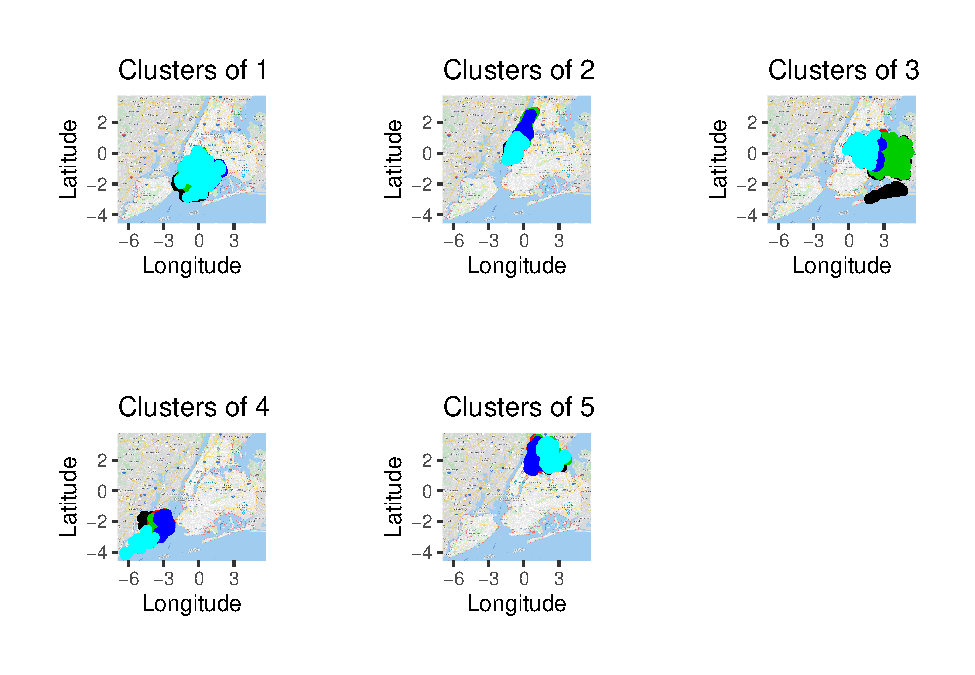
\includegraphics{project-code_files/figure-latex/unnamed-chunk-20-1.pdf}

\begin{Shaded}
\begin{Highlighting}[]
\KeywordTok{multiplots}\NormalTok{(all_cluster}\OperatorTok{$}\NormalTok{all_plot[}\DecValTok{6}\OperatorTok{:}\DecValTok{11}\NormalTok{], }\DataTypeTok{cols=}\DecValTok{3}\NormalTok{)}
\end{Highlighting}
\end{Shaded}

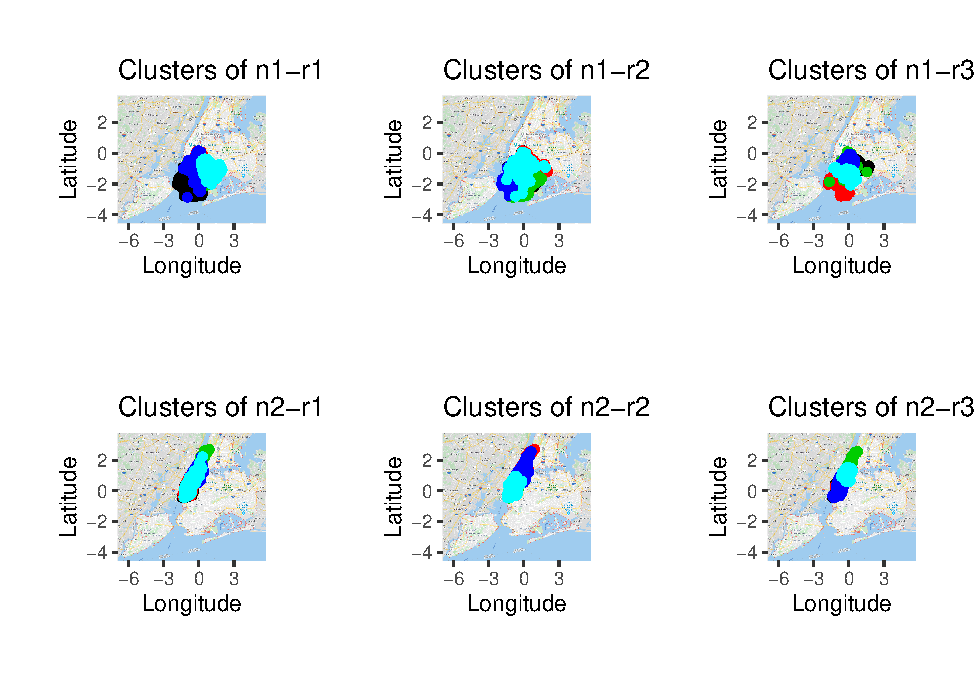
\includegraphics{project-code_files/figure-latex/unnamed-chunk-21-1.pdf}

\begin{Shaded}
\begin{Highlighting}[]
\KeywordTok{multiplots}\NormalTok{(all_cluster}\OperatorTok{$}\NormalTok{all_plot[}\DecValTok{12}\OperatorTok{:}\DecValTok{17}\NormalTok{], }\DataTypeTok{cols=}\DecValTok{3}\NormalTok{)}
\end{Highlighting}
\end{Shaded}

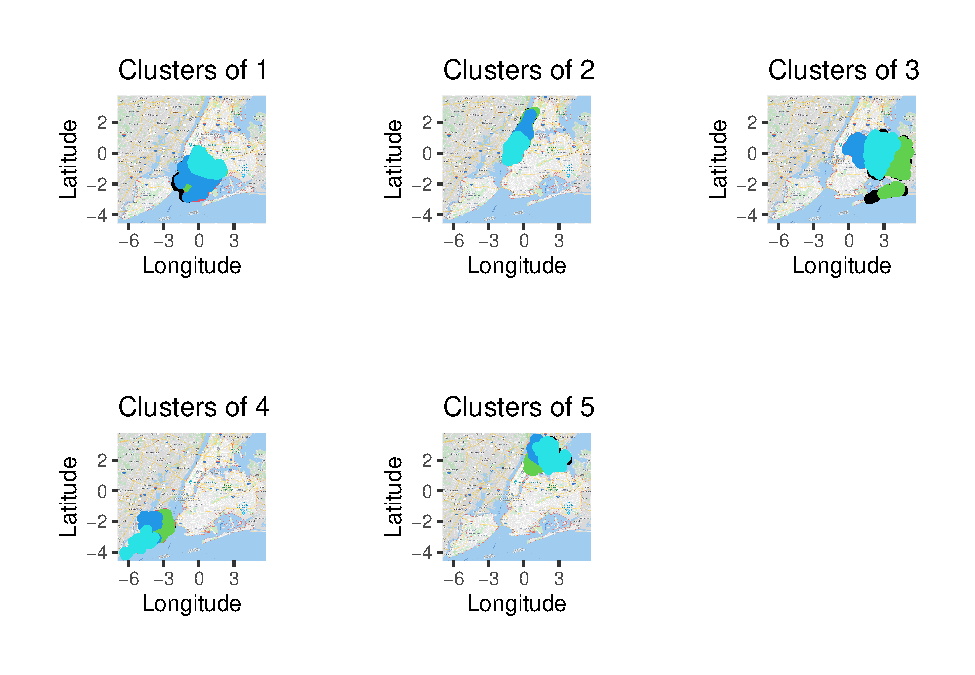
\includegraphics{project-code_files/figure-latex/unnamed-chunk-22-1.pdf}

\begin{Shaded}
\begin{Highlighting}[]
\KeywordTok{multiplots}\NormalTok{(all_cluster}\OperatorTok{$}\NormalTok{all_plot[}\KeywordTok{c}\NormalTok{(}\DecValTok{18}\OperatorTok{:}\DecValTok{20}\NormalTok{,}\DecValTok{22}\NormalTok{,}\DecValTok{23}\NormalTok{)], }\DataTypeTok{cols=}\DecValTok{3}\NormalTok{)}
\end{Highlighting}
\end{Shaded}

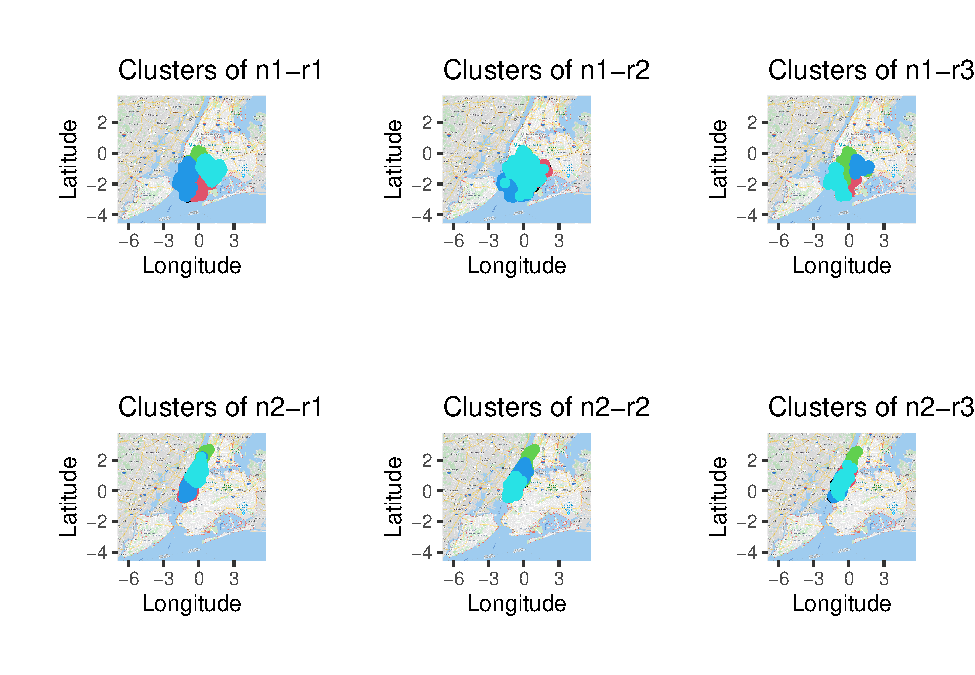
\includegraphics{project-code_files/figure-latex/unnamed-chunk-23-1.pdf}

\begin{verbatim}
## NULL
## NULL
\end{verbatim}

\hypertarget{pcamixdata}{%
\section{PCAmixdata}\label{pcamixdata}}

\begin{Shaded}
\begin{Highlighting}[]
\CommentTok{## Split mixed dataset into quantitative and qualitative variables}
\CommentTok{## For now excluding the target variable "Churn", which will be added later as a supplementary variable}
\CommentTok{#split <- splitmix(dataset[1:5])}

\NormalTok{split =}\StringTok{ }\KeywordTok{splitmix}\NormalTok{(clust_data}\OperatorTok{$}\NormalTok{all)}
\CommentTok{## PCA}
\NormalTok{res.pcamix <-}\StringTok{ }\KeywordTok{PCAmix}\NormalTok{(}\DataTypeTok{X.quanti=}\NormalTok{split}\OperatorTok{$}\NormalTok{X.quanti,  }
                     \DataTypeTok{X.quali=}\NormalTok{split}\OperatorTok{$}\NormalTok{X.quali, }
                     \DataTypeTok{rename.level=}\OtherTok{TRUE}\NormalTok{, }
                     \DataTypeTok{graph=}\OtherTok{FALSE}\NormalTok{, }
                     \DataTypeTok{ndim=}\DecValTok{25}\NormalTok{)}

\NormalTok{res.pcamix}
\end{Highlighting}
\end{Shaded}

\begin{verbatim}
## 
## Call:
## PCAmix(X.quanti = split$X.quanti, X.quali = split$X.quali, ndim = 25,     rename.level = TRUE, graph = FALSE)
## 
## Method = Principal Component of mixed data (PCAmix)
## 
## 
## "name" "description"
## "$eig" "eigenvalues of the principal components (PC) "
## "$ind" "results for the individuals (coord,contrib,cos2)"
## "$quanti" "results for the quantitative variables (coord,contrib,cos2)"
## "$levels" "results for the levels of the qualitative variables (coord,contrib,cos2)"
## "$quali" "results for the qualitative variables (contrib,relative contrib)"
## "$sqload" "squared loadings"
## "$coef" "coef of the linear combinations defining the PC"
\end{verbatim}

eig.val \textless- get\_eigenvalue(res.famd) head(eig.val)

fviz\_screeplot(res.famd)

\begin{Shaded}
\begin{Highlighting}[]
\CommentTok{## Inspect principal components}
\NormalTok{res.pcamix}\OperatorTok{$}\NormalTok{eig}
\end{Highlighting}
\end{Shaded}

\begin{verbatim}
##       Eigenvalue Proportion Cumulative
## dim 1  2.1303801  23.670890   23.67089
## dim 2  1.8046238  20.051375   43.72227
## dim 3  1.2456603  13.840670   57.56294
## dim 4  1.0028761  11.143067   68.70600
## dim 5  0.9971611  11.079568   79.78557
## dim 6  0.9570021  10.633357   90.41893
## dim 7  0.4201255   4.668061   95.08699
## dim 8  0.2652652   2.947391   98.03438
## dim 9  0.1769058   1.965620  100.00000
\end{verbatim}

\begin{Shaded}
\begin{Highlighting}[]
\CommentTok{# Use Scree Diagram to select the components:}
\KeywordTok{plot}\NormalTok{(res.pcamix}\OperatorTok{$}\NormalTok{eig, }\DataTypeTok{type=}\StringTok{"b"}\NormalTok{, }\DataTypeTok{main=}\StringTok{"Scree Diagram"}\NormalTok{, }\DataTypeTok{xlab=}\StringTok{"Number of Component"}\NormalTok{, }\DataTypeTok{ylab=}\StringTok{"Eigenvalues"}\NormalTok{)}
\KeywordTok{abline}\NormalTok{(}\DataTypeTok{h=}\DecValTok{1}\NormalTok{, }\DataTypeTok{lwd=}\DecValTok{3}\NormalTok{, }\DataTypeTok{col=}\StringTok{"red"}\NormalTok{)}
\end{Highlighting}
\end{Shaded}

\includegraphics{project-code_files/figure-latex/unnamed-chunk-26-1.pdf}

\hypertarget{hierarchical-cluster-analysis}{%
\section{Hierarchical Cluster
Analysis}\label{hierarchical-cluster-analysis}}

\begin{Shaded}
\begin{Highlighting}[]
\NormalTok{agg =}\StringTok{ }\KeywordTok{aggregate}\NormalTok{(price }\OperatorTok{~}\NormalTok{neighbourhood_group}\OperatorTok{+}\NormalTok{room_type, clust_data}\OperatorTok{$}\NormalTok{all , mean)}


\NormalTok{name_hc =}\StringTok{ }\KeywordTok{c}\NormalTok{()}
\ControlFlowTok{for}\NormalTok{ (n1 }\ControlFlowTok{in} \KeywordTok{unique}\NormalTok{(agg}\OperatorTok{$}\NormalTok{neighbourhood_group))}
\NormalTok{\{}
  \ControlFlowTok{for}\NormalTok{(n2 }\ControlFlowTok{in} \KeywordTok{unique}\NormalTok{(agg}\OperatorTok{$}\NormalTok{room_type))}
\NormalTok{  \{}
\NormalTok{    name_hc =}\StringTok{ }\KeywordTok{c}\NormalTok{(name_hc, }\KeywordTok{paste0}\NormalTok{(n1,}\StringTok{"/"}\NormalTok{,n2))}
\NormalTok{  \}}
\NormalTok{\}}
\KeywordTok{rownames}\NormalTok{(agg) =}\StringTok{ }\NormalTok{name_hc}

\NormalTok{agg}
\end{Highlighting}
\end{Shaded}

\begin{verbatim}
##                               neighbourhood_group       room_type       price
## Brooklyn/Private room                    Brooklyn    Private room -0.68331638
## Brooklyn/Entire home/apt                Manhattan    Private room -0.31844499
## Brooklyn/Shared room                       Queens    Private room -0.73368292
## Manhattan/Private room              Staten Island    Private room -0.78758723
## Manhattan/Entire home/apt                   Bronx    Private room -0.79719615
## Manhattan/Shared room                    Brooklyn Entire home/apt  0.32170945
## Queens/Private room                     Manhattan Entire home/apt  0.82148490
## Queens/Entire home/apt                     Queens Entire home/apt  0.08237678
## Queens/Shared room                  Staten Island Entire home/apt -0.07711867
## Staten Island/Private room                  Bronx Entire home/apt -0.10379804
## Staten Island/Entire home/apt            Brooklyn     Shared room -0.93711857
## Staten Island/Shared room               Manhattan     Shared room -0.53647655
## Bronx/Private room                         Queens     Shared room -0.93058224
## Bronx/Entire home/apt               Staten Island     Shared room -0.77955083
## Bronx/Shared room                           Bronx     Shared room -0.95841842
\end{verbatim}

\begin{Shaded}
\begin{Highlighting}[]
\NormalTok{gower <-}\StringTok{ }\KeywordTok{daisy}\NormalTok{(agg, }\DataTypeTok{metric =} \StringTok{"gower"}\NormalTok{)}
\NormalTok{hc1 <-}\StringTok{ }\KeywordTok{hclust}\NormalTok{(gower, }\DataTypeTok{method =} \StringTok{"complete"}\NormalTok{ )}

\KeywordTok{plot}\NormalTok{(hc1, }\DataTypeTok{cex =} \FloatTok{0.6}\NormalTok{, }\DataTypeTok{hang =} \DecValTok{-1}\NormalTok{)}
\end{Highlighting}
\end{Shaded}

\includegraphics{project-code_files/figure-latex/unnamed-chunk-27-1.pdf}

\begin{Shaded}
\begin{Highlighting}[]
\NormalTok{avg_dend_obj <-}\StringTok{ }\KeywordTok{as.dendrogram}\NormalTok{(hc1)}
\NormalTok{avg_col_dend <-}\StringTok{ }\KeywordTok{color_branches}\NormalTok{(avg_dend_obj, }\DataTypeTok{h =} \FloatTok{0.6}\NormalTok{)}
\KeywordTok{plot}\NormalTok{(avg_col_dend, }\DataTypeTok{cex=} \FloatTok{0.6}\NormalTok{)}
\end{Highlighting}
\end{Shaded}

\includegraphics{project-code_files/figure-latex/unnamed-chunk-28-1.pdf}

\begin{Shaded}
\begin{Highlighting}[]
\NormalTok{agg =}\StringTok{ }\KeywordTok{aggregate}\NormalTok{(price }\OperatorTok{~}\NormalTok{neighbourhood_group, clust_data}\OperatorTok{$}\NormalTok{all , mean)}
\NormalTok{agg}
\end{Highlighting}
\end{Shaded}

\begin{verbatim}
##   neighbourhood_group      price
## 1            Brooklyn -0.2147398
## 2           Manhattan  0.3601591
## 3              Queens -0.4396243
## 4       Staten Island -0.4574125
## 5               Bronx -0.5650283
\end{verbatim}

\begin{Shaded}
\begin{Highlighting}[]
\KeywordTok{rownames}\NormalTok{(agg) =}\StringTok{ }\KeywordTok{c}\NormalTok{(}\StringTok{"Brooklyn"}\NormalTok{,}\StringTok{"Manhattan"}\NormalTok{,}
                  \StringTok{"Queens"}\NormalTok{,}\StringTok{"Staten Island"}\NormalTok{, }\StringTok{"Bronx"}\NormalTok{)}
\NormalTok{agg}\OperatorTok{$}\NormalTok{neighbourhood_group =}\StringTok{ }\OtherTok{NULL}
\NormalTok{gower <-}\StringTok{ }\KeywordTok{daisy}\NormalTok{(agg, }\DataTypeTok{metric =} \StringTok{"gower"}\NormalTok{)}
\NormalTok{hc1 <-}\StringTok{ }\KeywordTok{hclust}\NormalTok{(gower, }\DataTypeTok{method =} \StringTok{"complete"}\NormalTok{ )}

\KeywordTok{plot}\NormalTok{(hc1, }\DataTypeTok{cex =} \FloatTok{0.6}\NormalTok{, }\DataTypeTok{hang =} \DecValTok{-1}\NormalTok{)}
\end{Highlighting}
\end{Shaded}

\includegraphics{project-code_files/figure-latex/unnamed-chunk-29-1.pdf}

\begin{Shaded}
\begin{Highlighting}[]
\CommentTok{#clust <- cutree(hc1, k = 5)}

\CommentTok{#fviz_cluster(list(data = agg, cluster = clust))  ## from ‘factoextra’ package }
\end{Highlighting}
\end{Shaded}

\hypertarget{section}{%
\section{==========================================}\label{section}}

DA VEDEREE

\hypertarget{factor-analysis-of-mixed-data-famd}{%
\section{- Factor Analysis of Mixed Data
(FAMD)}\label{factor-analysis-of-mixed-data-famd}}

\url{http://www.sthda.com/english/articles/31-principal-component-methods-in-r-practical-guide/115-famd-factor-analysis-of-mixed-data-in-r-essentials/}
\url{https://nextjournal.com/pc-methods/calculate-pc-mixed-data}
\url{https://cran.r-project.org/web/packages/FactoMineR/index.html}
\url{https://stats.stackexchange.com/questions/5774/can-principal-component-analysis-be-applied-to-datasets-containing-a-mix-of-cont}

\begin{Shaded}
\begin{Highlighting}[]
\KeywordTok{library}\NormalTok{(}\StringTok{"FactoMineR"}\NormalTok{)}
\KeywordTok{library}\NormalTok{(}\StringTok{"factoextra"}\NormalTok{)}
\end{Highlighting}
\end{Shaded}

FAMD (base, ncp = 5, sup.var = NULL, ind.sup = NULL, graph = TRUE) -
base : a data frame with n rows (individuals) and p columns (variables).
- ncp: the number of dimensions kept in the results (by default 5) -
sup.var: a vector indicating the indexes of the supplementary variables.
- ind.sup: a vector indicating the indexes of the supplementary
individuals. - graph : a logical value. If TRUE a graph is displayed.

\begin{Shaded}
\begin{Highlighting}[]
\NormalTok{res.famd <-}\StringTok{ }\KeywordTok{FAMD}\NormalTok{(clust_data}\OperatorTok{$}\NormalTok{all, }\DataTypeTok{graph =}\NormalTok{ F, }\DataTypeTok{ncp =} \DecValTok{5}\NormalTok{)}
\KeywordTok{print}\NormalTok{(res.famd)}
\end{Highlighting}
\end{Shaded}

\begin{verbatim}
## *The results are available in the following objects:
## 
##   name          description                             
## 1 "$eig"        "eigenvalues and inertia"               
## 2 "$var"        "Results for the variables"             
## 3 "$ind"        "results for the individuals"           
## 4 "$quali.var"  "Results for the qualitative variables" 
## 5 "$quanti.var" "Results for the quantitative variables"
\end{verbatim}

\begin{Shaded}
\begin{Highlighting}[]
\NormalTok{eig.val <-}\StringTok{ }\KeywordTok{get_eigenvalue}\NormalTok{(res.famd)}
\KeywordTok{head}\NormalTok{(eig.val)}
\end{Highlighting}
\end{Shaded}

\begin{verbatim}
##       eigenvalue variance.percent cumulative.variance.percent
## Dim.1  2.1303801         23.67089                    23.67089
## Dim.2  1.8046238         20.05138                    43.72227
## Dim.3  1.2456603         13.84067                    57.56294
## Dim.4  1.0028761         11.14307                    68.70600
## Dim.5  0.9971611         11.07957                    79.78557
\end{verbatim}

\begin{Shaded}
\begin{Highlighting}[]
\KeywordTok{fviz_screeplot}\NormalTok{(res.famd)}
\end{Highlighting}
\end{Shaded}

\includegraphics{project-code_files/figure-latex/unnamed-chunk-32-1.pdf}

\begin{Shaded}
\begin{Highlighting}[]
\NormalTok{quanti.var <-}\StringTok{ }\KeywordTok{get_famd_var}\NormalTok{(res.famd, }\StringTok{"quanti.var"}\NormalTok{)}
\NormalTok{quanti.var}
\end{Highlighting}
\end{Shaded}

\begin{verbatim}
## FAMD results for quantitative variables 
##  ===================================================
##   Name       Description                      
## 1 "$coord"   "Coordinates"                    
## 2 "$cos2"    "Cos2, quality of representation"
## 3 "$contrib" "Contributions"
\end{verbatim}

\begin{Shaded}
\begin{Highlighting}[]
\KeywordTok{fviz_famd_var}\NormalTok{(res.famd, }\StringTok{"quanti.var"}\NormalTok{, }\DataTypeTok{col.var =} \StringTok{"contrib"}\NormalTok{, }
             \DataTypeTok{gradient.cols =} \KeywordTok{c}\NormalTok{(}\StringTok{"#00AFBB"}\NormalTok{, }\StringTok{"#E7B800"}\NormalTok{, }\StringTok{"#FC4E07"}\NormalTok{),}
             \DataTypeTok{repel =} \OtherTok{TRUE}\NormalTok{)}
\end{Highlighting}
\end{Shaded}

\includegraphics{project-code_files/figure-latex/unnamed-chunk-33-1.pdf}

\begin{Shaded}
\begin{Highlighting}[]
\NormalTok{quali.var <-}\StringTok{ }\KeywordTok{get_famd_var}\NormalTok{(res.famd, }\StringTok{"quali.var"}\NormalTok{)}
\NormalTok{quali.var }
\end{Highlighting}
\end{Shaded}

\begin{verbatim}
## FAMD results for qualitative variable categories 
##  ===================================================
##   Name       Description                      
## 1 "$coord"   "Coordinates"                    
## 2 "$cos2"    "Cos2, quality of representation"
## 3 "$contrib" "Contributions"
\end{verbatim}

\begin{Shaded}
\begin{Highlighting}[]
\KeywordTok{fviz_famd_var}\NormalTok{(res.famd, }\StringTok{"quali.var"}\NormalTok{, }\DataTypeTok{col.var =} \StringTok{"contrib"}\NormalTok{, }
             \DataTypeTok{gradient.cols =} \KeywordTok{c}\NormalTok{(}\StringTok{"#00AFBB"}\NormalTok{, }\StringTok{"#E7B800"}\NormalTok{, }\StringTok{"#FC4E07"}\NormalTok{)}
\NormalTok{             )}
\end{Highlighting}
\end{Shaded}

\includegraphics{project-code_files/figure-latex/unnamed-chunk-34-1.pdf}

ind \textless- get\_famd\_ind(res.famd) ind

fviz\_famd\_ind(res.famd, col.ind = ``cos2'', gradient.cols =
c(``\#00AFBB'', ``\#E7B800'', ``\#FC4E07''), repel = TRUE)

\begin{Shaded}
\begin{Highlighting}[]
\NormalTok{var <-}\StringTok{ }\KeywordTok{get_famd_var}\NormalTok{(res.famd)}
\NormalTok{var}
\end{Highlighting}
\end{Shaded}

\begin{verbatim}
## FAMD results for variables 
##  ===================================================
##   Name       Description                      
## 1 "$coord"   "Coordinates"                    
## 2 "$cos2"    "Cos2, quality of representation"
## 3 "$contrib" "Contributions"
\end{verbatim}

\begin{Shaded}
\begin{Highlighting}[]
\CommentTok{# Coordinates of variables}
\KeywordTok{head}\NormalTok{(var}\OperatorTok{$}\NormalTok{coord)}
\end{Highlighting}
\end{Shaded}

\begin{verbatim}
##                          Dim.1       Dim.2      Dim.3        Dim.4        Dim.5
## latitude            0.03892236 0.799743946 0.04903898 0.0016811055 0.0018258497
## longitude           0.58030735 0.126293692 0.16517205 0.0001203636 0.0001685452
## price               0.51607212 0.005313173 0.23572672 0.0005079180 0.0001842764
## neighbourhood_group 0.63900709 0.871714919 0.43427934 0.5273304673 0.4806939587
## room_type           0.35607121 0.001558062 0.36144319 0.4732362202 0.5142884950
\end{verbatim}

\begin{Shaded}
\begin{Highlighting}[]
\CommentTok{# Cos2: quality of representation on the factore map}
\KeywordTok{head}\NormalTok{(var}\OperatorTok{$}\NormalTok{cos2)}
\end{Highlighting}
\end{Shaded}

\begin{verbatim}
##                          Dim.1        Dim.2       Dim.3        Dim.4
## latitude            0.00151495 6.395904e-01 0.002404821 2.826116e-06
## longitude           0.33675663 1.595010e-02 0.027281805 1.448739e-08
## price               0.26633043 2.822981e-05 0.055567086 2.579807e-07
## neighbourhood_group 0.10208251 1.899717e-01 0.047149637 6.951936e-02
## room_type           0.06339335 1.213779e-06 0.065320588 1.119763e-01
##                            Dim.5
## latitude            3.333727e-06
## longitude           2.840749e-08
## price               3.395780e-08
## neighbourhood_group 5.776667e-02
## room_type           1.322463e-01
\end{verbatim}

\begin{Shaded}
\begin{Highlighting}[]
\CommentTok{# Contributions to the  dimensions}
\KeywordTok{head}\NormalTok{(var}\OperatorTok{$}\NormalTok{contrib)}
\end{Highlighting}
\end{Shaded}

\begin{verbatim}
##                         Dim.1       Dim.2     Dim.3       Dim.4       Dim.5
## latitude             1.827015 44.31638047  3.936786  0.16762844  0.18310478
## longitude           27.239615  6.99833910 13.259799  0.01200184  0.01690250
## price               24.224415  0.29441998 18.923837  0.05064614  0.01848011
## neighbourhood_group 29.994980 48.30452324 34.863386 52.58181750 48.20624738
## room_type           16.713975  0.08633722 29.016193 47.18790608 51.57526523
\end{verbatim}

\begin{Shaded}
\begin{Highlighting}[]
\CommentTok{# Plot of variables}
\KeywordTok{fviz_famd_var}\NormalTok{(res.famd, }\DataTypeTok{repel =} \OtherTok{TRUE}\NormalTok{)}
\end{Highlighting}
\end{Shaded}

\includegraphics{project-code_files/figure-latex/unnamed-chunk-37-1.pdf}

\begin{Shaded}
\begin{Highlighting}[]
\CommentTok{# Contribution to the first dimension}
\KeywordTok{fviz_contrib}\NormalTok{(res.famd, }\StringTok{"var"}\NormalTok{, }\DataTypeTok{axes =} \DecValTok{1}\NormalTok{)}
\end{Highlighting}
\end{Shaded}

\includegraphics{project-code_files/figure-latex/unnamed-chunk-37-2.pdf}

\begin{Shaded}
\begin{Highlighting}[]
\CommentTok{# Contribution to the second dimension}
\KeywordTok{fviz_contrib}\NormalTok{(res.famd, }\StringTok{"var"}\NormalTok{, }\DataTypeTok{axes =} \DecValTok{2}\NormalTok{)}
\end{Highlighting}
\end{Shaded}

\includegraphics{project-code_files/figure-latex/unnamed-chunk-37-3.pdf}

\begin{Shaded}
\begin{Highlighting}[]
\CommentTok{# Contribution to the third dimension}
\KeywordTok{fviz_contrib}\NormalTok{(res.famd, }\StringTok{"var"}\NormalTok{, }\DataTypeTok{axes =} \DecValTok{3}\NormalTok{)}
\end{Highlighting}
\end{Shaded}

\includegraphics{project-code_files/figure-latex/unnamed-chunk-37-4.pdf}

\begin{Shaded}
\begin{Highlighting}[]
\CommentTok{# Contribution to the forth dimension}
\KeywordTok{fviz_contrib}\NormalTok{(res.famd, }\StringTok{"var"}\NormalTok{, }\DataTypeTok{axes =} \DecValTok{4}\NormalTok{)}
\end{Highlighting}
\end{Shaded}

\includegraphics{project-code_files/figure-latex/unnamed-chunk-37-5.pdf}

\begin{Shaded}
\begin{Highlighting}[]
\CommentTok{# Contribution to the fifth dimension}
\KeywordTok{fviz_contrib}\NormalTok{(res.famd, }\StringTok{"var"}\NormalTok{, }\DataTypeTok{axes =} \DecValTok{5}\NormalTok{)}
\end{Highlighting}
\end{Shaded}

\includegraphics{project-code_files/figure-latex/unnamed-chunk-37-6.pdf}

\begin{Shaded}
\begin{Highlighting}[]
\CommentTok{# Contribution to the sixth dimension}
\CommentTok{#fviz_contrib(res.famd, "var", axes = 6)}
\CommentTok{# Contribution to the seventh dimension}
\CommentTok{#fviz_contrib(res.famd, "var", axes = 7)}
\CommentTok{# Contribution to the eighth dimension}
\CommentTok{#fviz_contrib(res.famd, "var", axes = 8)}
\end{Highlighting}
\end{Shaded}

\end{document}
